% IEEE Transactions on Robotics / Mechatronics Template
\documentclass[lettersize,journal]{IEEEtran}

% Packages
\usepackage{amsmath,amssymb,amsfonts}
\usepackage{algorithmic}
\usepackage{algorithm}
\usepackage{array}
\usepackage[caption=false,font=normalsize,labelfont=sf,textfont=sf]{subfig}
\usepackage{textcomp}
\usepackage{stfloats}
\usepackage{url}
\usepackage{verbatim}
\usepackage{graphicx}
\usepackage{cite}
\usepackage{xcolor}
\usepackage{booktabs}
\usepackage{multirow}
\usepackage{bm}
% \usepackage[inkscapelatex=false]{svg}

% Figure path
\graphicspath{{figures/}}

% Correct hyphenation
\hyphenation{op-tical net-works semi-conduc-tor IEEE-Xplore}

% ============================================================================
% COMPILATION INSTRUCTIONS:
% 1. Ensure all figures are in the 'figures/' directory
% 2. Compile with: pdflatex paper_dr_rma.tex
% 3. Run bibtex if needed: bibtex paper_dr_rma
% 4. Compile twice more for cross-references
%
% Required figures (to be created or referenced):
% - fig1_system_overview.pdf (system diagram + architecture)
% - fig1_attention_heatmap.png (attention weights over time)
% - fig2_inertia_estimation.png (true vs estimated inertia)
% - baseline_comparison_test2_inertia_steps.png (tracking comparison)
% ============================================================================

\begin{document} 

\title{DR-RMA: Dual-Rate Rapid Motor Adaptation Control for Series Elastic Actuators with Time-Varying Inertia} 

\author{Xiubo Xia, Xiaoyu Geng, Yongling Fu, Donghao Jia, Jian Sun
    \thanks{Xiubo Xia, Jian Sun are with the School of Mechanical Engineering and Automation, Beihang University, Beijing, China, (e-mail:xiaxiubo@buaa.edu.cn; buaasunjian@buaa.edu.cn)} 
}

\maketitle 

\begin{abstract}
Series Elastic Actuators (SEAs) are widely employed in collaborative robots, rehabilitation robots, and physical 
human-robot interaction systems due to their inherent compliance and force control capabilities. 
However, achieving robust control of SEAs remains challenging under abrupt load-inertia changes, 
such as those caused by payload switching or dynamic manipulation tasks.
Conventional model-based controllers rely heavily on accurate system parameters, 
making them vulnerable to large and abrupt inertia variations, 
whereas adaptive methods may suffer from estimation lag during fast transients. 
This paper presents DR-RMA (Dual-Rate Rapid Motor Adaptation), 
a novel learning-based control framework that enables robust SEA trajectory tracking under abrupt load-inertia variations.
The proposed architecture contains two parallel adaptation branches with different operating rates: 
a dual-timescale Fast Attention v2 Branch that estimates bounded load inertia from measurable SEA history, 
enabling attention redistribution within one 5 ms control step; and a Slow Temporal 
Convolutional Network (TCN) Branch that extracts implicit friction- and hysteresis-related features over 
longer time horizons.
Through teacher-student distillation, DR-RMA eliminates the dependency on privileged ground-truth parameters 
during deployment. Simulation results on a rotational SEA with extreme inertia transients demonstrate that 
DR-RMA achieves an RMSE of 0.0176 rad in the extreme inertia-transient test, outperforming RMA, PPO, PD-DOB, and LQR baselines. 
These results indicate that the proposed DR-RMA improves both tracking accuracy 
and transient robustness under large and abrupt load-inertia variations.
\end{abstract}

\begin{IEEEkeywords}
Series Elastic Actuator, Learning-based Control, Rapid Motor Adaptation, Attention Mechanism, 
Load Inertia Estimation, Time-Varying Inertia, Robust Trajectory Tracking
\end{IEEEkeywords}

\section{Introduction}

\IEEEPARstart{S}{eries} Elastic Actuators have emerged as a cornerstone technology in physical human-robot interaction applications, including collaborative manipulators~\cite{li2024Advances}, lower-limb exoskeletons~\cite{hang2025Design}, and prosthetic devices~\cite{fagioli2024Underactuated}. By introducing a compliant element between the motor and load, SEAs provide inherent force control capabilities, impact tolerance, and energy storage—properties that are essential for safe and efficient interaction with humans and unstructured environments. However, the control of SEAs becomes significantly more challenging when the load inertia varies during operation, a common scenario in manipulation tasks involving payload changes, human-robot collaboration with varying contact forces, or assistive devices adapting to different users and terrains.

This issue becomes particularly important for future assistive and companion robots that operate in elderly-care, rehabilitation, and home environments. In such settings, robots are expected to share space with non-expert users, manipulate daily objects, support human limbs, and react safely to unexpected events. When a manipulator suddenly picks up a heavy object, releases an object, or loses a payload during motion, the effective inertia reflected to an SEA joint can change abruptly. A controller that is tuned only for nominal inertia may then produce excessive torque, excite elastic oscillations, or temporarily lose tracking accuracy. These transient behaviors are not merely performance degradations; in close human-robot coexistence, they directly affect interaction safety, comfort, and trust. Therefore, maintaining stable and predictable SEA behavior under abrupt inertia changes is a key requirement for deploying compliant robots in human-centered environments.

\begin{figure}[ht]
    \centering
    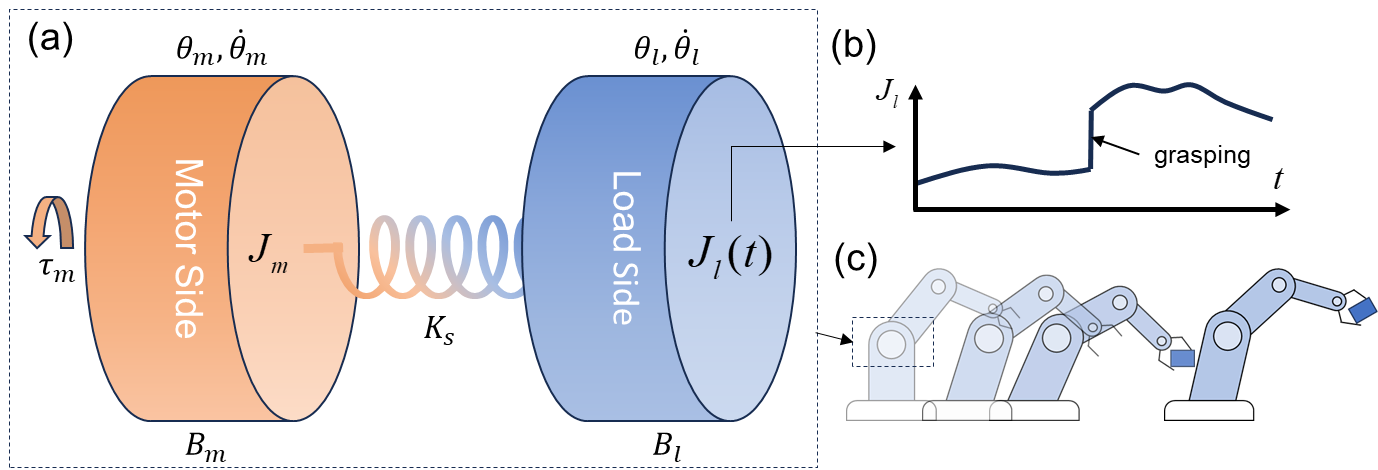
\includegraphics [width=0.48\textwidth]{figs/fig1png.png}
    \caption{Overview of the Series Elastic Actuator (SEA) control 
    problem addressed in this work. \textbf{(a)} Schematic of a 
    rotational SEA joint. The motor side , with inertia $J_m$,
    and the load side, with time-varying inertia $J_l(t)$, are 
    mechanically coupled through a compliant torsional spring with 
    stiffness $K_s$. The motor applies torque $\tau_m$, while the 
    motor-side and load-side angular positions, $\theta_m$ and 
    $\theta_l$, are measured independently. Their difference, 
    $\Delta\theta = \theta_m - \theta_l$, represents the spring 
    deflection and is directly related to the transmitted torque.
     \textbf{(b)} Illustrative application 
    scenario: a robotic manipulator equipped with SEA joints 
    performs pick-and-place tasks with payloads of different 
    masses. As the payload changes over time (top curve), the 
    effective load inertia $J_l(t)$ undergoes abrupt step-like 
    variations spanning more than one order of magnitude. These rapid 
    inertia transients, together with the coupled 
    motor--spring--load dynamics of SEAs, severely degrade the performance 
    of conventional model-based and fixed-gain controllers, 
    motivating the proposed DR-RMA framework.}
    \label{fig:sea_overview}
\end{figure}

Since their introduction for safe physical human-robot interaction~\cite{pratt1995Series, pratt1999Series}, SEA control has largely focused on the trade-off among mechanical compliance, control bandwidth, and force/position tracking accuracy~\cite{calanca2016Review, paine2014Design}. Classical cascaded position-force control and impedance-control designs~\cite{hogan1985Impedance} can achieve satisfactory performance when the plant is close to its nominal model. However, the same compliance that improves interaction safety also creates coupled motor-spring-load dynamics whose resonant frequency and damping ratio depend on the load inertia. When SEAs are embedded in flexible or multi-body systems, such as anthropomorphic robotic arms~\cite{li2024Advances}, this coupling becomes more sensitive to payload-dependent parameter mismatch. As a result, abrupt load changes can simultaneously shift the dominant dynamics and invalidate the fixed parameters used in nominal controller design.

Conventional model-based controllers, including Linear Quadratic Regulators (LQR)~\cite{sariyildiz2026Robust} and model predictive control (MPC)~\cite{zhang2024Development}, rely on an accurate model or a sufficiently representative linearization. These approaches remain attractive because their stability and constraint-handling properties are relatively transparent, yet their performance can degrade rapidly when the true inertia deviates from the design value. Robust and observer-based methods reduce this sensitivity by estimating lumped disturbances or compensating unmodeled dynamics. Disturbance-observer-based SEA control has been used to improve disturbance rejection and output stiffness~\cite{asignacion2021high, ito2024disturbance}, and recent variants include variable disturbance observers~\cite{sun2025Variablea} and nonlinear DOBs for multi-joint systems~\cite{han2021nonlinear}. Impedance and admittance strategies have also been refined for uncertain interaction tasks~\cite{lee2021hybrid, ozdemir2025adaptive, zhong2021toward}, while ADRC and sliding-mode methods provide additional robustness margins~\cite{chen2021practical, sun2021trajectory}.

Adaptive methods explicitly estimate changing parameters or update controller gains online. Adaptive observers and parameter-estimation schemes have been incorporated into SEA control loops~\cite{song2025adaptive, min2026adaptive}, and hybrid adaptive control~\cite{lanh2023Hybrid} and $\mathcal{L}_1$ adaptive resonance ratio control~\cite{min2024L1adaptive} further improve robustness to structured uncertainty. Nevertheless, abrupt inertia transients remain challenging for these methods. Observer bandwidths cannot be increased arbitrarily without amplifying noise, adaptation laws require sufficient excitation, and aggressive gain updates can excite the SEA elastic mode. Therefore, even when steady-state robustness is good, the transient interval immediately after payload attachment or release may still show estimation lag, overshoot, or conservative control action.

Learning-based control provides an alternative route by learning policies directly from interaction data rather than relying solely on analytical models. PPO~\cite{schulman2017Proximal} and related deep-RL methods have been applied to SEA force control, dynamic performance improvement, and high-performance control~\cite{sambhus2023real, lahmann2025series, xia2026high}. Neural dynamic models and learning-augmented MPC have also been explored for nonlinear SEA behavior~\cite{umurzakov2025neural, zhang2024Development}, while learning-based whole-body controllers have enabled SEA-equipped mobile manipulators to perform complex tasks~\cite{liu2021whole, ren2022integrated}. These results show the potential of data-driven methods for complex compliant systems, but a monolithic RL policy often generalizes poorly to unseen physical parameters unless the training distribution is broad enough or the controller has an explicit adaptation mechanism.

The Rapid Motor Adaptation (RMA) framework~\cite{kumar2021RMA} addresses this generalization problem using teacher-student training: a teacher policy observes privileged physical parameters during training, while a student module estimates latent factors from observation history for deployment. This paradigm is well suited to sim-to-real transfer because privileged quantities are not required at run time. However, existing RMA variants typically encode history through a single temporal module, which mixes fast-changing quantities, such as load inertia, with slower effects, such as friction, hysteresis, and stiffness mismatch. This motivates an architecture that separates rapid explicit parameter estimation from slower latent-dynamics inference. DR-RMA therefore decouples explicit fast inertia estimation from slower implicit dynamics through a dual-timescale Fast Attention v2 Branch and a Slow TCN Branch.

\subsection{Contributions}

This paper presents DR-RMA (Dual-Rate Rapid Motor Adaptation), a control architecture for SEAs with time-varying inertia. The key contributions are:

\begin{enumerate}
\item \textbf{Dual-Rate Adaptation}: We decouple fast load-inertia estimation from slower implicit dynamics using a dual-timescale attention branch and a TCN branch.

\item \textbf{Attention Collapse}: We identify an emergent attention-concentration behavior that reacts to inertia changes within one 5 ms control step.

\item \textbf{Evaluation}: We validate DR-RMA in fixed-inertia and extreme inertia-transient simulations, achieving 0.0176 rad RMSE in the transient test and outperforming PPO, RMA, PD+DOB, and LQR baselines.
\end{enumerate}

The remainder of this paper is organized as follows. Section~II formulates the control problem and presents the SEA dynamics. Section~III details the DR-RMA architecture, including the teacher policy, dual-rate student networks, and training methodology. Section~IV describes the simulation experimental setup and baseline controllers. Section~V presents comprehensive simulation results including attention mechanism analysis and baseline comparisons. Section~VI discusses key findings and limitations. Section~VII describes the hardware experimental testbench for future physical validation. Section~VIII concludes the paper.

\section{Problem Formulation}

\subsection{SEA System Dynamics}

The fundamental physical challenge addressed in this work is illustrated in Fig. \ref{fig:sea_overview}. As shown in Fig. \ref{fig:sea_overview}(a), the SEA is conventionally modeled as a two-mass system consisting of a motor and a load, coupled by a compliant spring element. However, unlike traditional nominal models that assume constant physical properties, the load inertia $J_l(t)$ in our formulation is explicitly defined as a time-varying parameter to reflect practical dynamic manipulation tasks. The system dynamics can be described by the following coupled differential equations:

\begin{equation}
\begin{aligned}
J_m \ddot{\theta}_m &= \tau_m - K_s(\theta_m - \theta_l) - B_m\dot{\theta}_m - \tau_{f,m}, \\
J_l \ddot{\theta}_l &= K_s(\theta_m - \theta_l) - B_l\dot{\theta}_l - \tau_{f,l}.
\end{aligned}
\label{eq:sea_dynamics}
\end{equation}

\noindent where $\theta_m$ and $\theta_l$ are the motor and load angular positions (rad), $J_m$ and $J_l$ are the motor and load inertias (kg·m$^2$), $\tau_m$ is the motor torque (N·m), $K_s$ is the spring stiffness (N·m/rad), $B_m$ and $B_l$ are viscous damping coefficients (N·m·s/rad), and $\tau_{f,m}$ and $\tau_{f,l}$ represent Coulomb friction torques (N·m).
In this study, load-inertia variations are modeled as piecewise-constant payload changes caused by attachment, release, or clutch engagement events. Between two events, $J_l$ is constant and the standard two-inertia SEA dynamics in~\eqref{eq:sea_dynamics} are used. At the switching instant, the inertia change is treated as an external hybrid event applied between discrete control updates; impact dynamics and momentum exchange during the infinitesimal transition are not modeled explicitly. Therefore, the additional $\dot{J}_l\dot{\theta}_l$ term associated with continuously moving mass redistribution is outside the scope of the nominal model. This assumption matches the simulation benchmark and the planned clutch-based testbench, where the controller is evaluated on recovery after discrete inertia transitions rather than on the detailed contact mechanics of the switching event.

As depicted in Fig. \ref{fig:sea_overview}(a) and (b), when an anthropomorphic robotic manipulator executes a routine grasping operation, the system experiences an instantaneous step increase in load inertia upon payload contact. These abrupt parameter transients—often coupled with unmodeled frictional variations—fundamentally alter the system's resonant frequency and coupled dynamics. Such discontinuous distribution shifts cause traditional linear controllers and slow-converging adaptive methods to exhibit severe performance degradation, motivating the need for the rapid, dual-rate adaptation architecture proposed in this paper.


\begin{figure*}[t]
\centering
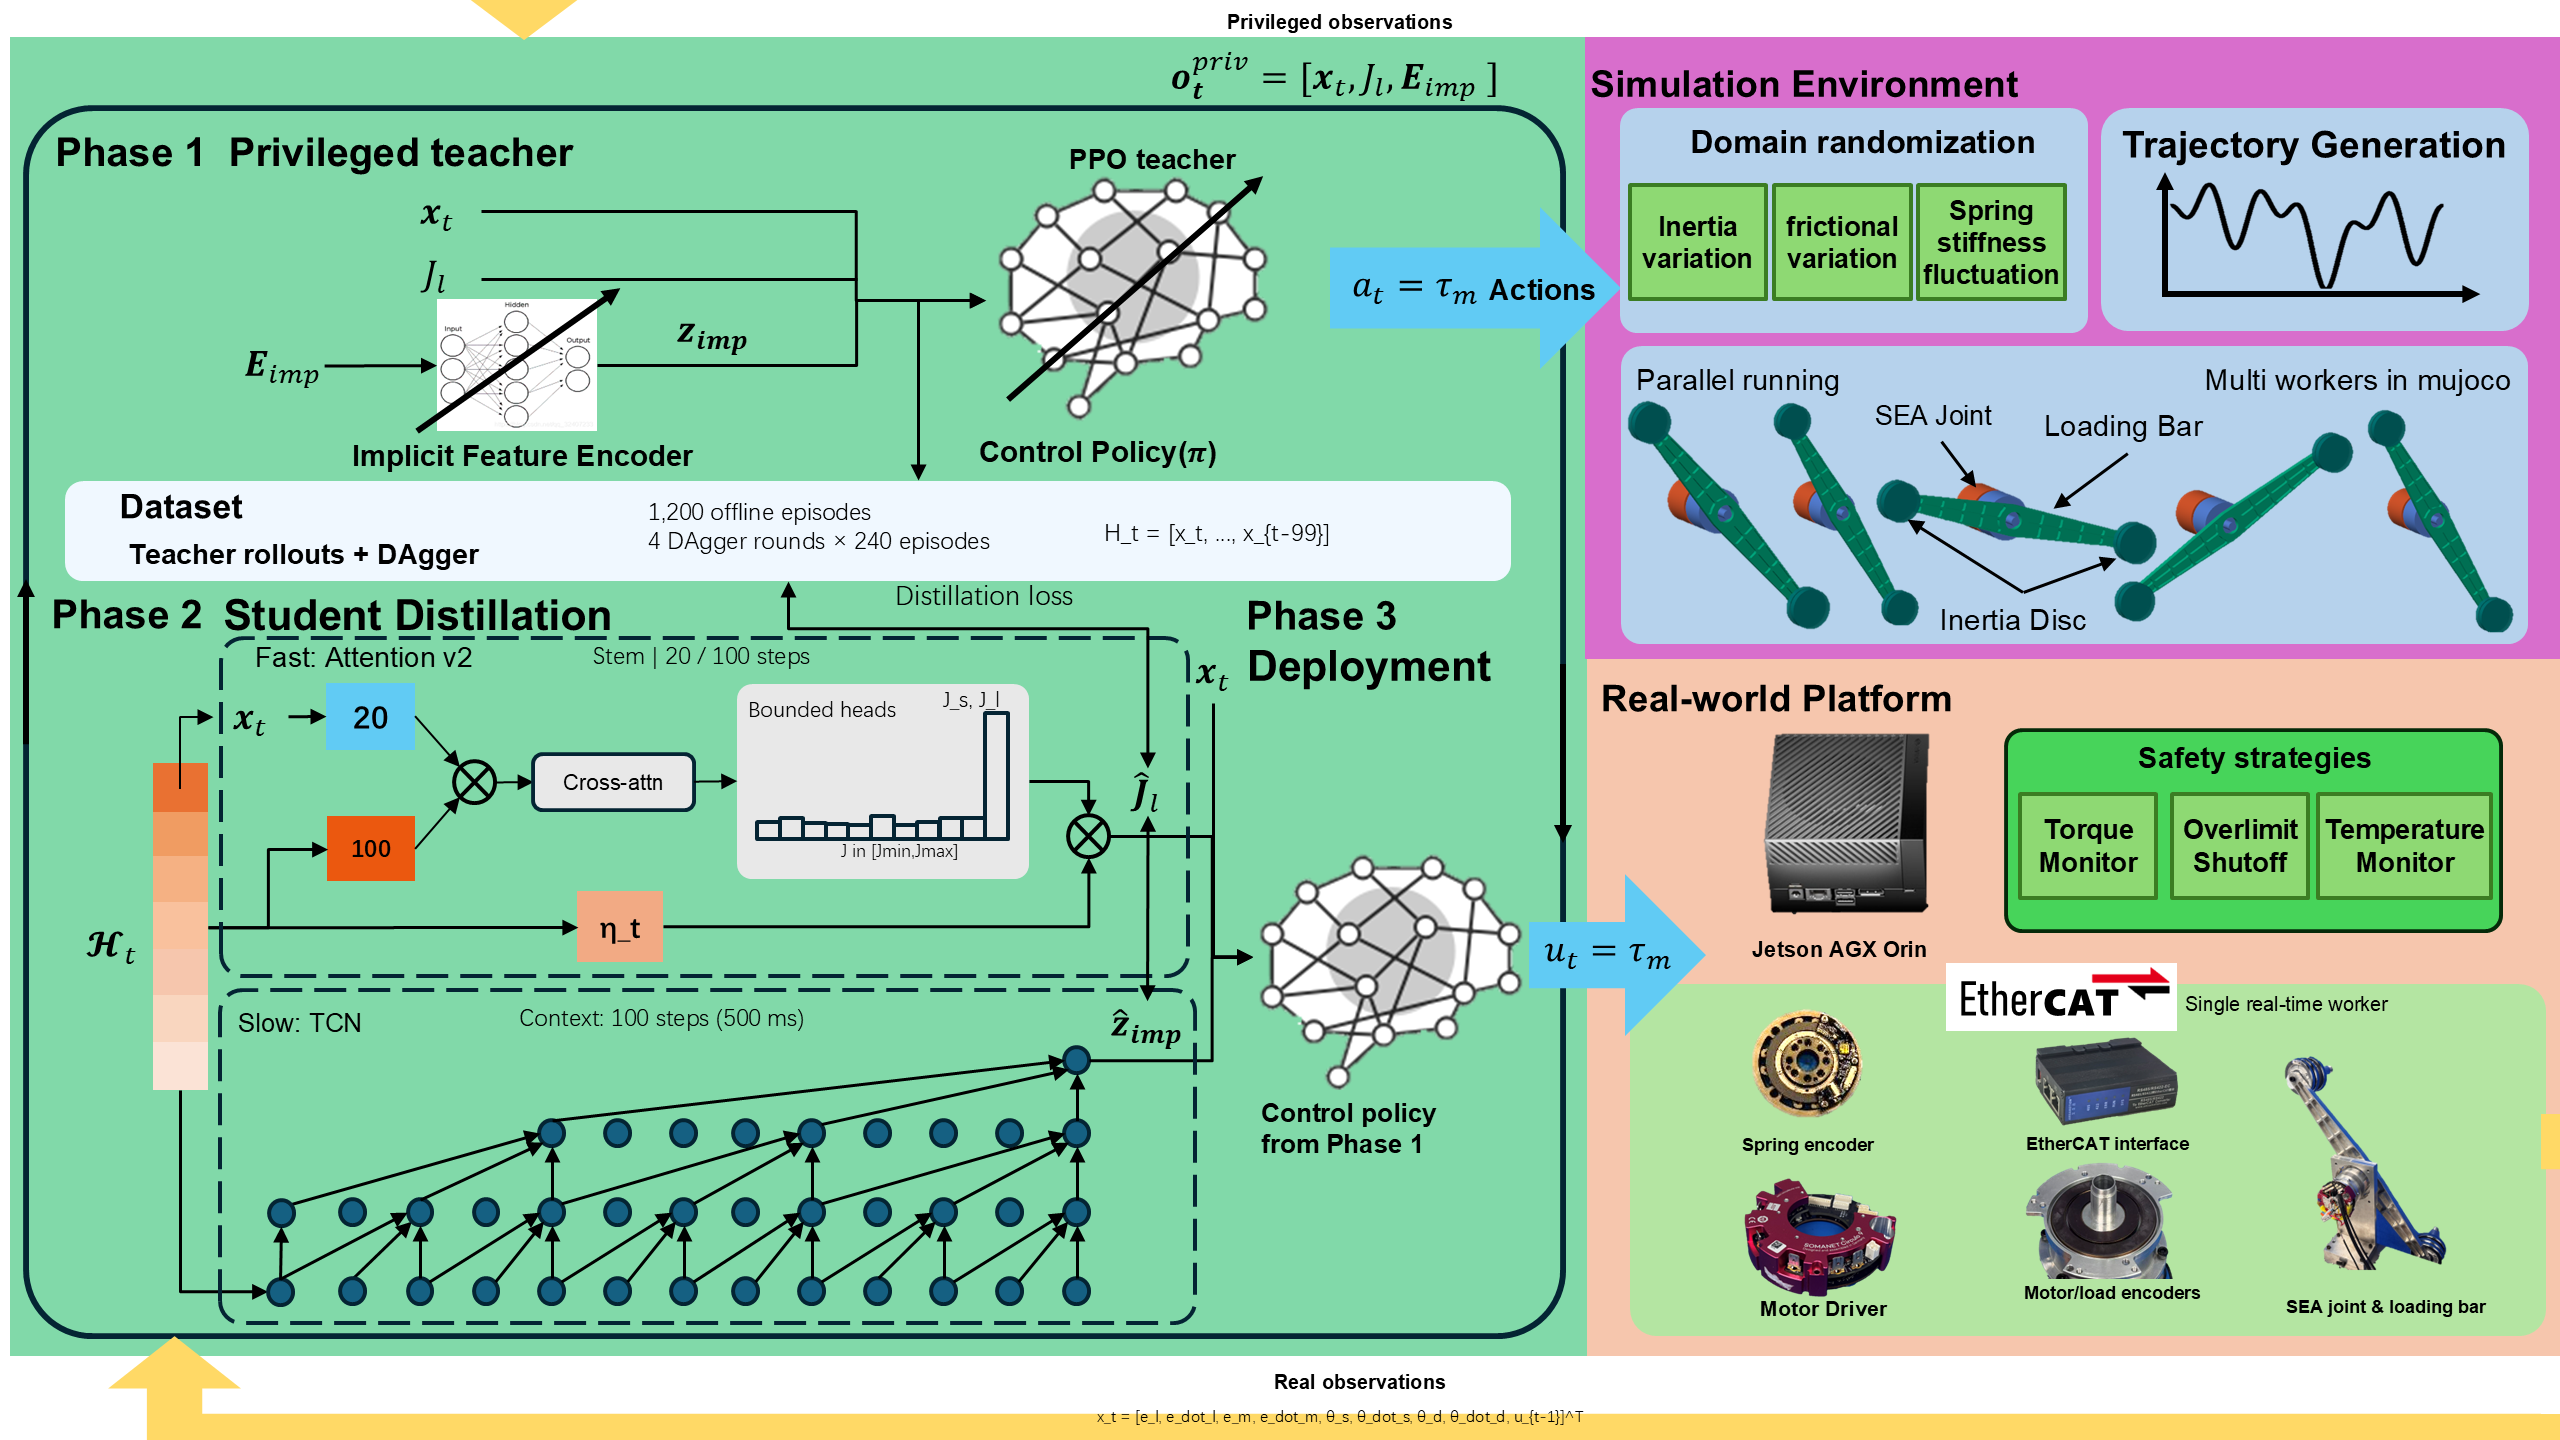
\includegraphics[width=0.96\textwidth]{figs/fig2png.png}
\caption{The complete architecture and deployment pipeline of the proposed DR-RMA framework. The paradigm consists of three main phases. \textbf{Phase 1 (Teacher Training):} A teacher policy (PPO agent) is trained in a simulated environment with domain randomization, utilizing privileged observations that include ground-truth inertia $J_l$ and implicit features $E_{imp}$ extracted via an encoder. \textbf{Phase 2 (Student Distillation):} The trained teacher policy is frozen to collect a dataset of history-to-parameter mappings. A dual-rate student network is then trained via supervised learning: a dual-timescale Fast Attention v2 branch estimates explicit bounded inertia $\hat{J}_l$ from measurable dynamics history, while a Slow TCN branch processes a 100-step history window (500 ms at 200 Hz) to estimate implicit dynamics $\hat{z}_{imp}$. \textbf{Phase 3 (Zero-Shot Deployment):} The student networks and the frozen teacher policy are designed for zero-shot deployment on real-world hardware. The system operates strictly on the non-privileged observation history $\mathcal{H}_t$, enabling rapid adaptation to extreme inertia transients without requiring privileged parameters during deployment.}
\label{fig:dr_rma_architecture}
\end{figure*}


The spring deflection $\Delta\theta = \theta_m - \theta_l$ provides a measure of the transmitted torque:
\begin{equation}
\tau_s = K_s \Delta\theta \label{eq:spring_torque}
\end{equation}

\subsection{Time-Varying Inertia Challenge}

In practical applications, the load inertia $J_l(t)$ varies due to payload changes, human-robot interaction forces, or dynamic manipulation tasks. We consider the scenario where:
\begin{equation}
J_l(t) \in [J_{\min}, J_{\max}], \quad \frac{J_{\max}}{J_{\min}} \gg 1 \label{eq:inertia_range}
\end{equation}

In our experiments, $J_l(t) \in [0.05, 1.0]$ kg·m$^2$, representing a 20× variation range. The controller has no prior knowledge of when the discrete inertia transitions occur or which value will follow each transition.

\subsection{Control Objective}

Given a desired trajectory $\theta_d(t)$ and its derivatives $\dot{\theta}_d(t)$, $\ddot{\theta}_d(t)$, the control objective is to design a feedback controller that computes motor torque $\tau_m(t)$ such that the load position $\theta_l(t)$ tracks the reference with minimal error:
\begin{equation}
\min_{\tau_m} \int_0^T \left[ w_p(\theta_l - \theta_d)^2 + w_v(\dot{\theta}_l - \dot{\theta}_d)^2 + w_u \tau_m^2 \right] dt \label{eq:objective}
\end{equation}

\noindent subject to torque constraints $|\tau_m| \leq \tau_{\max}$ and stability requirements.

\subsection{Observation Space}

The controller has access to the following 9-dimensional observation vector at each control timestep:
\begin{equation}
\bm{x}_t = \begin{bmatrix}
e_{l} & \dot{e}_{l} & e_{m} & \dot{e}_{m} & \theta_s & \dot{\theta}_s & \theta_d & \dot{\theta}_d & u_{t-1}
\end{bmatrix}^\mathrm{T} \label{eq:observation}
\end{equation}

\noindent where $e_{l} = \theta_d - \theta_l$ and $\dot{e}_{l} = \dot{\theta}_d - \dot{\theta}_l$ are load-side tracking errors, $e_{m} = \theta_d - \theta_m$ and $\dot{e}_{m} = \dot{\theta}_d - \dot{\theta}_m$ are motor-side tracking errors with respect to the same reference trajectory, $\theta_s$ and $\dot{\theta}_s$ are spring deflection and rate, $\theta_d$ and $\dot{\theta}_d$ are reference position and velocity, and $u_{t-1} \in [-1, 1]$ is the previous normalized control action.

Critically, the observation does not include the load inertia $J_l$ or friction parameters, which must be estimated from observation history.

\subsection{Key Challenges}

Controlling SEAs with time-varying inertia presents several fundamental challenges:

\begin{enumerate}
\item \textbf{History-Based Estimation}: Traditional inertia estimators rely on measuring acceleration $\ddot{\theta}_l$. However, during trajectory tracking with smooth references, acceleration can be small over parts of the cycle, making inertia weakly observable from instantaneous measurements alone. DR-RMA therefore uses a finite observation history and depends on the excitation provided by the commanded trajectory and closed-loop response, rather than claiming inertia identifiability under arbitrary zero-excitation conditions.

\item \textbf{Rapid Adaptation}: When inertia changes abruptly (e.g., payload drop), the controller must detect and adapt within milliseconds to prevent tracking errors from accumulating.

\item \textbf{Multi-Timescale Dynamics}: Inertia changes occur on fast timescales (10-100ms), while friction and hysteresis evolve slowly (100-1000ms). A single adaptation mechanism may not effectively capture both phenomena.

\item \textbf{Deployment Constraints}: Real-time control at 200 Hz requires end-to-end inference latency below the 5 ms control period and memory footprint suitable for embedded systems.
\end{enumerate}

DR-RMA addresses these challenges through a dual-rate architecture that explicitly separates fast inertia estimation from slow implicit feature extraction, as detailed in Section~III.

\section{DR-RMA Architecture}

The DR-RMA framework consists of two training phases: (1) a teacher policy trained with privileged information using reinforcement learning, and (2) dual-rate student networks trained via supervised distillation to estimate the privileged information from observation history. Fig.~\ref{fig:dr_rma_architecture} illustrates the complete architecture.

\subsection{Teacher Policy with Privileged Information}

\subsubsection{Privileged Observation Space}

During training, the teacher policy has access to privileged information that is unavailable during deployment:
\begin{equation}
\bm{o}_t^{\text{priv}} = \begin{bmatrix}
\bm{x}_t^\mathrm{T} & J_l & \bm{E}_{\text{imp}}^\mathrm{T}
\end{bmatrix}^\mathrm{T} \in \mathbb{R}^{15} \label{eq:priv_obs}
\end{equation}

\noindent where $\bm{x}_t \in \mathbb{R}^9$ is the base observation (Eq.~\ref{eq:observation}), $J_l \in \mathbb{R}$ is the ground-truth load inertia, and $\bm{E}_{\text{imp}} \in \mathbb{R}^5$ contains implicit parameters:
\begin{equation}
\bm{E}_{\text{imp}} = \begin{bmatrix}
\tau_{c,m} & \tau_{c,l} & B_m & B_l & \Delta K_s
\end{bmatrix}^\mathrm{T} \label{eq:implicit_params}
\end{equation}

\noindent representing motor and load Coulomb friction ($\tau_{c,m}$, $\tau_{c,l}$), viscous damping coefficients ($B_m$, $B_l$), and spring stiffness deviation ($\Delta K_s$).

\subsubsection{Implicit Feature Encoder}

To reduce dimensionality and extract relevant features from $\bm{E}_{\text{imp}}$, we employ a two-layer MLP encoder:
\begin{equation}
\begin{aligned}
\bm{h}_1 &= \text{ELU}(\bm{W}_1 \bm{E}_{\text{imp}} + \bm{b}_1), \quad \bm{W}_1 \in \mathbb{R}^{16 \times 5}, \\
\bm{z}_{\text{imp}} &= \bm{W}_2 \bm{h}_1 + \bm{b}_2, \quad \bm{W}_2 \in \mathbb{R}^{8 \times 16}.
\end{aligned}
\label{eq:encoder_z}
\end{equation}

\noindent where $\bm{z}_{\text{imp}} \in \mathbb{R}^8$ is the implicit feature vector. The teacher policy then operates on the 18-dimensional feature vector:
\begin{equation}
\bm{f}_t = \begin{bmatrix}
\bm{x}_t^\mathrm{T} & J_l & \bm{z}_{\text{imp}}^\mathrm{T}
\end{bmatrix}^\mathrm{T} \in \mathbb{R}^{18} \label{eq:teacher_features}
\end{equation}

\subsubsection{Policy Network}

The teacher policy is parameterized as a Gaussian policy:
\begin{equation}
\begin{aligned}
\bm{\mu}_t &= \pi_\theta(\bm{f}_t) = \text{MLP}(\bm{f}_t) \in \mathbb{R}, \\
u_t &\sim \mathcal{N}(\mu_t, \sigma^2).
\end{aligned}
\label{eq:teacher_policy}
\end{equation}

\noindent where the MLP consists of two hidden layers with 128 units each and ELU activations. The log standard deviation $\log \sigma$ is a learnable parameter initialized to $-0.5$.

\subsubsection{Training Objective}

The teacher policy is trained using Proximal Policy Optimization (PPO)~\cite{schulman2017Proximal} to maximize the expected return:
\begin{equation}
\mathcal{J}(\theta) = \mathbb{E}_{\tau \sim \pi_\theta} \left[ \sum_{t=0}^T \gamma^t r_t \right] \label{eq:ppo_objective}
\end{equation}

The reward function is designed to encourage accurate tracking while penalizing excessive control effort and vibrations:
\begin{align}
r_t = &\, r_{\text{alive}} + r_{\text{precision}} - w_p e_{l}^2 - w_v \dot{e}_{l}^2 \nonumber \\
&- w_s \theta_s^2 - w_u \tau_m^2 - w_{\Delta u} (\Delta \tau_m)^2 - w_{\ddot{\tau}_s} \ddot{\tau}_s^2 \label{eq:reward}
\end{align}

\noindent where $r_{\text{alive}} = 1.0$ encourages survival, $r_{\text{precision}} = 5.0 \exp(-e_{l}^2 / 0.01)$ provides a Gaussian bonus for high precision, and the penalty terms discourage position error ($w_p = 1.5$), velocity error ($w_v = 0.05$), spring deflection ($w_s = 1.0$), control effort ($w_u = 0.001$), control smoothness ($w_{\Delta u} = 0.005$), and spring torque jerk ($w_{\ddot{\tau}_s} = 0.001$). The anti-resonance term $\ddot{\tau}_s$ explicitly penalizes high-frequency vibrations.

Training is performed with 8 parallel environments for 2 million timesteps, with domain randomization over inertia ($J_l \in [0.05, 1.0]$ kg·m$^2$), friction parameters, and trajectory characteristics.

\subsection{Fast Attention v2 Branch for Inertia Estimation}

The Fast Attention v2 Branch estimates load inertia $\hat{J}_l$ from a history window of observations. Unlike purely instantaneous acceleration-based estimators, the attention mechanism uses recent input-output history to exploit the excitation present in the tested tracking trajectories. The deployed estimator uses only measurable SEA signals: load/motor velocities and finite-difference accelerations reconstructed from encoder data, spring deflection and spring velocity, spring torque computed from the measured deflection and nominal stiffness, and the previous action. It does not take load friction, motor friction, viscous damping, oracle inertia, or oracle latent features as inputs. Thus, the method is intended to improve inertia estimation under weak instantaneous acceleration without relying on privileged deployment-time parameters.

\subsubsection{History Window Construction}

At each timestep $t$, we maintain a FIFO queue of the most recent $L = 100$ observations:
\begin{equation}
\mathcal{H}_t = \{\bm{x}_{t-L+1}, \bm{x}_{t-L+2}, \ldots, \bm{x}_t\} \in \mathbb{R}^{L \times 9} \label{eq:history_window}
\end{equation}

The window length $L = 100$ corresponds to 0.5 seconds at 200 Hz control frequency, providing sufficient temporal context for inertia estimation while maintaining computational efficiency.

\subsubsection{Dual-Timescale Current-to-History Attention}

The v2 estimator first maps each observation history to an 8-dimensional measurable dynamics feature vector $\bm{\phi}_i$:
\begin{equation}
\begin{aligned}
\bm{\phi}_i = [&\dot{\theta}_{l,i}, \ddot{\theta}_{l,i}, \dot{\theta}_{m,i}, \ddot{\theta}_{m,i}, \\
&\theta_{s,i}, \dot{\theta}_{s,i}, \tau_{s,i}, u_{i-1}]^\mathrm{T}.
\end{aligned}
\label{eq:fast_features}
\end{equation}

\noindent The features are normalized by fixed physical scales before entering a temporal convolutional stem, which produces encoded tokens $\bm{e}_{t-L+1:t} \in \mathbb{R}^{L \times d}$. The most recent token serves as the query for two attention paths:
\begin{equation}
\begin{aligned}
\bm{c}_{s,t} &= \mathrm{MHA}_s(\bm{e}_t, \bm{e}_{t-L_s+1:t}, \bm{e}_{t-L_s+1:t}), \\
\bm{c}_{l,t} &= \mathrm{MHA}_l(\bm{e}_t, \bm{e}_{t-L+1:t}, \bm{e}_{t-L+1:t}),
\end{aligned}
\label{eq:dual_attention}
\end{equation}

\noindent where $L=100$, $L_s=20$, $d=128$, and each attention path uses 8 heads. The short path emphasizes rapid changes immediately after a payload event, whereas the long path preserves a broader temporal context for steady segments.

The short and long contexts are mapped to bounded inertia estimates and blended by a learned jump gate:
\begin{equation}
\begin{aligned}
\hat{J}_{s,t} &= J_{\min} + (J_{\max}-J_{\min})\sigma(g_s(\bm{c}_{s,t}, \bm{e}_t)), \\
\hat{J}_{\ell,t} &= J_{\min} + (J_{\max}-J_{\min})\sigma(g_l(\bm{c}_{l,t}, \bm{e}_t)), \\
\eta_t &= \sigma(g_\eta(\bm{c}_{s,t}, \bm{c}_{l,t}, \bm{e}_t)), \\
\hat{J}_t &= \eta_t \hat{J}_{s,t} + (1-\eta_t)\hat{J}_{\ell,t}.
\end{aligned}
\label{eq:inertia_estimate}
\end{equation}

\noindent The same gate head also outputs a confidence signal for diagnostics. However, the final deployment uses the raw blended estimate in~\eqref{eq:inertia_estimate}; a fixed hard confidence threshold is not used because it can indefinitely hold an outdated inertia value during low-excitation intervals.

\subsubsection{Attention Collapse Mechanism}

A key discovery of our work is the emergent attention collapse phenomenon. During steady-state operation with constant inertia, attention weights are distributed over the relevant history window. However, when the inertia changes abruptly, the attention weights concentrate on recent observations within a single control timestep (5 ms), and the jump gate shifts the estimator toward the short-timescale branch:
\begin{equation}
\alpha_{t,L} \rightarrow 1, \quad H(\bm{\alpha}) \rightarrow 0, \quad \eta_t \rightarrow 1.
\label{eq:attention_collapse}
\end{equation}

This collapse occurs because the current observation exhibits a distribution shift relative to the historical observations under the changed inertia, causing the attention mechanism to down-weight outdated information. Importantly, this adaptation is \emph{automatic}—no explicit change detection is required.

The Fast Attention v2 Branch is trained with a weighted regression loss together with auxiliary short-branch, long-branch, jump-gate, and confidence losses:
\begin{equation}
\mathcal{L}_{\text{fast}} =
\mathcal{L}_{\text{reg}} + \lambda_r \mathcal{L}_{\text{rel}}
+ \lambda_s \mathcal{L}_{s} + \lambda_l \mathcal{L}_{l}
+ \lambda_g \mathcal{L}_{g} + \lambda_c \mathcal{L}_{c}.
\label{eq:fast_loss}
\end{equation}

\noindent The regression terms supervise $\hat{J}_t$, $\hat{J}_{s,t}$, and $\hat{J}_{\ell,t}$ using ground-truth inertia labels, while the gate-related terms encourage the short-timescale path during detected inertia jumps and provide confidence as a diagnostic output.

\subsection{Slow TCN Branch for Implicit Feature Extraction}

While the Fast Attention v2 Branch focuses on rapid inertia estimation, the Slow TCN Branch extracts low-frequency implicit features such as friction and hysteresis that evolve over longer timescales.

\subsubsection{Causal Temporal Convolutional Network}

We employ a five-layer causal dilated convolutional network that processes the same history window $\mathcal{H}_t$. The input is first permuted to channel-first format $(B, 9, L)$ for 1D convolution.

Each layer consists of a causal convolution with dilation, layer normalization, and ELU activation:
\begin{equation}
\begin{aligned}
\bm{h}_1 &= \text{ELU}(\text{LN}(\text{Conv1D}_{d=1}^{k=8}(\mathcal{H}_t))) \in \mathbb{R}^{64 \times L}, \\
\bm{h}_2 &= \text{ELU}(\text{LN}(\text{Conv1D}_{d=2}^{k=8}(\bm{h}_1))) \in \mathbb{R}^{128 \times L}, \\
\bm{h}_3 &= \text{ELU}(\text{LN}(\text{Conv1D}_{d=4}^{k=8}(\bm{h}_2))) \in \mathbb{R}^{128 \times L}, \\
\bm{h}_4 &= \text{ELU}(\text{LN}(\text{Conv1D}_{d=8}^{k=4}(\bm{h}_3))) \in \mathbb{R}^{64 \times L}, \\
\bm{h}_5 &= \text{ELU}(\text{LN}(\text{Conv1D}_{d=16}^{k=4}(\bm{h}_4))) \in \mathbb{R}^{32 \times L}.
\end{aligned}
\label{eq:tcn_stack}
\end{equation}

\noindent where $k$ denotes kernel size and $d$ denotes dilation rate. Causal padding ensures that the output at time $t$ depends only on inputs up to time $t$, maintaining causality for real-time deployment.

The effective receptive field grows exponentially with dilation:
\begin{equation}
\text{RF} = 1 + \sum_{l=1}^5 d_l (k_l - 1) = 122 \text{ steps} \label{eq:receptive_field}
\end{equation}

Since the FIFO window contains 100 real observations, the effective real-data context is the full 100-step history, corresponding to 500 ms at 200 Hz. This horizon is sufficient to capture slow friction dynamics while remaining computationally efficient.

\subsubsection{Output Projection}

The final temporal feature at time $t$ is extracted and projected to the 8-dimensional implicit feature space:
\begin{equation}
\hat{\bm{z}}_{\text{imp}} = \bm{W}_{\text{out}} \bm{h}_5[:, -1] + \bm{b}_{\text{out}} \in \mathbb{R}^8 \label{eq:slow_output}
\end{equation}

\noindent where $\bm{h}_5[:, -1]$ selects the feature vector corresponding to the most recent timestep.

\subsubsection{Temporal Smoothing Loss}

To encourage smooth implicit feature estimates and suppress high-frequency noise, we augment the MSE loss with a temporal smoothing term:
\begin{equation}
\mathcal{L}_{\text{slow}} = \mathbb{E} \left[ \|\hat{\bm{z}}_{\text{imp}} - \bm{z}_{\text{imp}}\|^2 + \lambda \|\hat{\bm{z}}_{\text{imp}}^{(t)} - \hat{\bm{z}}_{\text{imp}}^{(t-1)}\|^2 \right] \label{eq:slow_loss}
\end{equation}

\noindent where $\lambda = 0.1$ balances accuracy and smoothness. This regularization reflects the physical intuition that friction parameters change slowly compared to inertia.

\subsection{Student Network Training}

\subsubsection{Data Collection}

After training the teacher policy to convergence, we freeze its parameters and collect a dataset by rolling out the teacher in diverse environments. For each episode, we record:
\begin{itemize}
\item History windows: $\mathcal{H}_t \in \mathbb{R}^{100 \times 9}$
\item Ground-truth inertia: $J_l \in \mathbb{R}$
\item Teacher's implicit features: $\bm{z}_{\text{imp}} \in \mathbb{R}^8$ (from Eq.~\ref{eq:encoder_z})
\end{itemize}

For the Fast Attention v2 Branch, we collect 1,200 teacher-rollout episodes with randomized friction and diverse trajectories, together with 120 independent validation episodes. The initial offline model is then refined using four rounds of on-policy DAgger, with the teacher blend factor annealed from $\beta=0.8$ to $0.5$, $0.2$, and finally $0.0$. Each DAgger round contributes 240 additional rollout episodes. This procedure exposes the estimator to the closed-loop state distribution induced by the student controller, rather than relying only on offline validation windows.

\subsubsection{Supervised Distillation}

The Fast and Slow branches are trained by supervised distillation and then integrated with the frozen teacher policy during deployment. The total student objective is
\begin{equation}
\mathcal{L}_{\text{total}} = \mathcal{L}_{\text{fast}} + \mathcal{L}_{\text{slow}} \label{eq:total_loss}
\end{equation}

The Fast Attention v2 model is selected using closed-loop evaluation rather than offline validation loss alone. Specifically, candidate checkpoints are evaluated on a suite of 108 independent conditions formed by 6 trajectory/inertia patterns, 6 Coulomb-friction levels, and 3 viscous-friction levels. The final deployment uses the raw bounded inertia estimate from~\eqref{eq:inertia_estimate}; the confidence output is retained for diagnostics but no hard confidence-hold threshold is applied.

\subsection{Deployment Pipeline}

During deployment, the complete inference pipeline is designed for the 200 Hz control loop:
\begin{enumerate}
\item Read 9D observation $\bm{x}_t$ from sensors
\item Update FIFO history buffer $\mathcal{H}_t$
\item Fast Attention v2 Branch: $\mathcal{H}_t \rightarrow \hat{J}_l$ (parallel)
\item Slow Branch: $\mathcal{H}_t \rightarrow \hat{\bm{z}}_{\text{imp}}$ (parallel)
\item Construct augmented observation: $\bm{f}_t = [\bm{x}_t^\mathrm{T}, \hat{J}_l, \hat{\bm{z}}_{\text{imp}}^\mathrm{T}]^\mathrm{T}$
\item Apply observation normalization (running mean/std from training)
\item Teacher policy: $\bm{f}_t \rightarrow u_t$
\item Denormalize and apply motor torque: $\tau_m = u_t \cdot \tau_{\max}$
\end{enumerate}

The Fast and Slow branches are structurally parallel. As discussed in Section~\ref{sec:computational_performance}, the exported ONNX control graph satisfies the 200 Hz real-time deadline in the tested single-thread CPU implementation.

\section{Experimental Setup}

\subsection{SEA System Specifications}

We evaluate DR-RMA in a high-fidelity MuJoCo simulation of a rotational SEA system. The system parameters are listed in Table~\ref{tab:system_params}.

\begin{table}[t]
\centering
\caption{SEA System Parameters}
\label{tab:system_params}
\begin{tabular}{@{}lcc@{}}
\toprule
Parameter & Symbol & Value \\
\midrule
Motor inertia & $J_m$ & 0.01 kg·m$^2$ \\
Load inertia (base) & $J_{l,\text{base}}$ & 0.04 kg·m$^2$ \\
Load inertia (range) & $J_l$ & [0.05, 1.0] kg·m$^2$ \\
Spring stiffness & $K_s$ & 3800 N·m/rad \\
Motor damping & $B_m$ & 0.0955 N·m·s/rad \\
Load damping & $B_l$ & 0.1 N·m·s/rad \\
Max motor torque & $\tau_{\max}$ & 61.0 N·m \\
Control frequency & $f_c$ & 200 Hz \\
Simulation timestep & $\Delta t_{\text{sim}}$ & 0.001 s (1000 Hz) \\
\bottomrule
\end{tabular}
\end{table}

The load inertia is varied using a payload slider mechanism based on the parallel axis theorem: $J_l = J_{l,\text{base}} + J_{\text{payload}} + m_{\text{payload}} r^2$, where $r$ is the slider position. This mechanism enables both smooth continuous variations and instantaneous step changes in inertia.

\subsection{Training Methodology}

\subsubsection{Phase 1: Teacher Policy Training}

The teacher policy is trained using PPO with the following configuration:
\begin{itemize}
\item Parallel environments: 8 (DummyVecEnv)
\item Total timesteps: 2,000,000
\item Rollout steps per environment: 1024
\item Mini-batch size: 128
\item Optimization epochs per rollout: 10
\item Learning rate: $3 \times 10^{-4}$
\item Discount factor $\gamma$: 0.99
\item GAE parameter $\lambda$: 0.95
\item PPO clip range: 0.2
\item Entropy coefficient: 0.01
\end{itemize}

Domain randomization is applied over:
\begin{itemize}
\item Inertia: $J_l \sim \mathcal{U}(0.05, 1.0)$ kg·m$^2$
\item Coulomb friction: $\tau_{c,m} \sim \mathcal{U}(0, 0.5)$ N·m, $\tau_{c,l} \sim \mathcal{U}(0, 0.3)$ N·m
\item Viscous damping: $B_m \sim \mathcal{U}(0.05, 0.3)$ N·m·s/rad, $B_l \sim \mathcal{U}(0, 0.1)$ N·m·s/rad
\item Spring stiffness deviation: $\Delta K_s \sim \mathcal{U}(-500, 500)$ N·m/rad
\item Trajectory amplitude: $A \sim \mathcal{U}(0.1, 1.2)$ rad
\item Trajectory frequency: $f \sim \mathcal{U}(0.1, 1.5)$ Hz
\end{itemize}

Inertia variation modes include constant, step changes (1-3 per episode), and sinusoidal variations (frequency 0.02-0.5 Hz).

\subsubsection{Phase 2: Student Network Training}

Data collection: 3,000 episodes using the frozen teacher policy, from which $\sim$150,000 history windows are subsampled for supervised training.

Training configuration:
\begin{itemize}
\item Optimizer: Adam
\item Initial learning rate: $10^{-3}$
\item Scheduler: CosineAnnealingLR (100 epochs)
\item Batch size: 512
\item Validation split: 10\%
\item Early stopping: patience 10 epochs
\end{itemize}

\subsection{Baseline Controllers}

We compare DR-RMA against four baseline controllers representing different control paradigms:

\subsubsection{PPO Baseline}

Pure Proximal Policy Optimization (PPO) trained with the same 9-dimensional observation space as DR-RMA's base observation, but without privileged information or adaptation modules. This represents a standard model-free RL approach that must learn a single fixed policy across all inertia variations.

\subsubsection{RMA Baseline}

The original Rapid Motor Adaptation framework~\cite{kumar2021RMA} using a single TCN-based adaptation module to estimate an 8-dimensional latent feature vector from observation history. Unlike DR-RMA's dual-rate design, RMA uses a unified temporal processing architecture without explicit inertia estimation.

\subsubsection{PD with Disturbance Observer (PD+DOB)}

The PD+DOB controller combines proportional-derivative feedback with a disturbance observer for robustness:
\begin{equation}
\begin{aligned}
\tau_m &= K_p e_{p,l} + K_d e_{v,l} + \tau_{\text{ff}} - \hat{\tau}_{\text{dist}}, \\
\hat{\tau}_{\text{dist}} &= \text{LPF}\left(J_{\text{nom}} \left(\frac{\tau_m - K_s \Delta\theta}{J_{\text{nom}}} - \ddot{\theta}_l\right)\right).
\end{aligned}
\label{eq:pddob_control}
\end{equation}

\noindent where $K_p = 85$, $K_d = 60$, $J_{\text{nom}} = 0.3$ kg·m$^2$, DOB gain $g_{\text{DOB}} = -6.5$, and the disturbance estimate is updated via discrete integration. The feedforward term $\tau_{\text{ff}} = J_{\text{nom}} \ddot{\theta}_d$ compensates for reference acceleration.

\subsubsection{Linear Quadratic Regulator (LQR)}

The LQR controller is designed based on the linearized SEA dynamics around the nominal inertia $J_{\text{nom}} = 0.3$ kg·m$^2$. The state vector is $\bm{x}_{\text{LQR}} = [e_{p,l}, e_{v,l}, \Delta\theta, \dot{\Delta\theta}]^\mathrm{T}$, and the control law is:
\begin{equation}
\tau_m = -\bm{K}_{\text{LQR}} \bm{x}_{\text{LQR}} \label{eq:lqr_control}
\end{equation}

The LQR gain $\bm{K}_{\text{LQR}}$ is computed by solving the continuous-time algebraic Riccati equation with cost matrices $\bm{Q} = \text{diag}(10, 1, 40, 1)$ and $R = 20.0$. These parameters were carefully tuned to balance tracking performance and torque smoothness, prioritizing control effort penalty to avoid saturation.

\subsection{Test Scenarios}

We evaluate all controllers on two test scenarios:

\textbf{Test 1: Fixed-Inertia Tracking} — Fixed inertia $J_l = 0.45$ kg·m$^2$ with sinusoidal reference trajectory (amplitude 0.5 rad, frequency 0.3 Hz) for 10 seconds. This tests baseline tracking performance without parameter variations.

\textbf{Test 2: Extreme Inertia Transients} — Initial inertia $J_l = 0.3$ kg·m$^2$ with two abrupt step changes representing extreme manipulation scenarios:
\begin{itemize}
\item $t = 3.0$ s: $J_l = 0.3 \rightarrow 0.05$ kg·m$^2$ (-83\%, payload release)
\item $t = 7.0$ s: $J_l = 0.05 \rightarrow 0.75$ kg·m$^2$ (+1400\%, heavy payload grasp)
\end{itemize}

The same sinusoidal reference is used. This scenario tests rapid adaptation capability under extreme parameter variations.

All tests use identical random seeds for fair comparison.

\section{Results and Analysis}

\subsection{Attention Mechanism Behavior}

We first analyze the attention collapse phenomenon during inertia step changes in Test 2. Fig.~\ref{fig:attention_heatmap} shows the attention weight distribution over time, with clear vertical bands at the two inertia change events.

\begin{figure}[t]
\centering
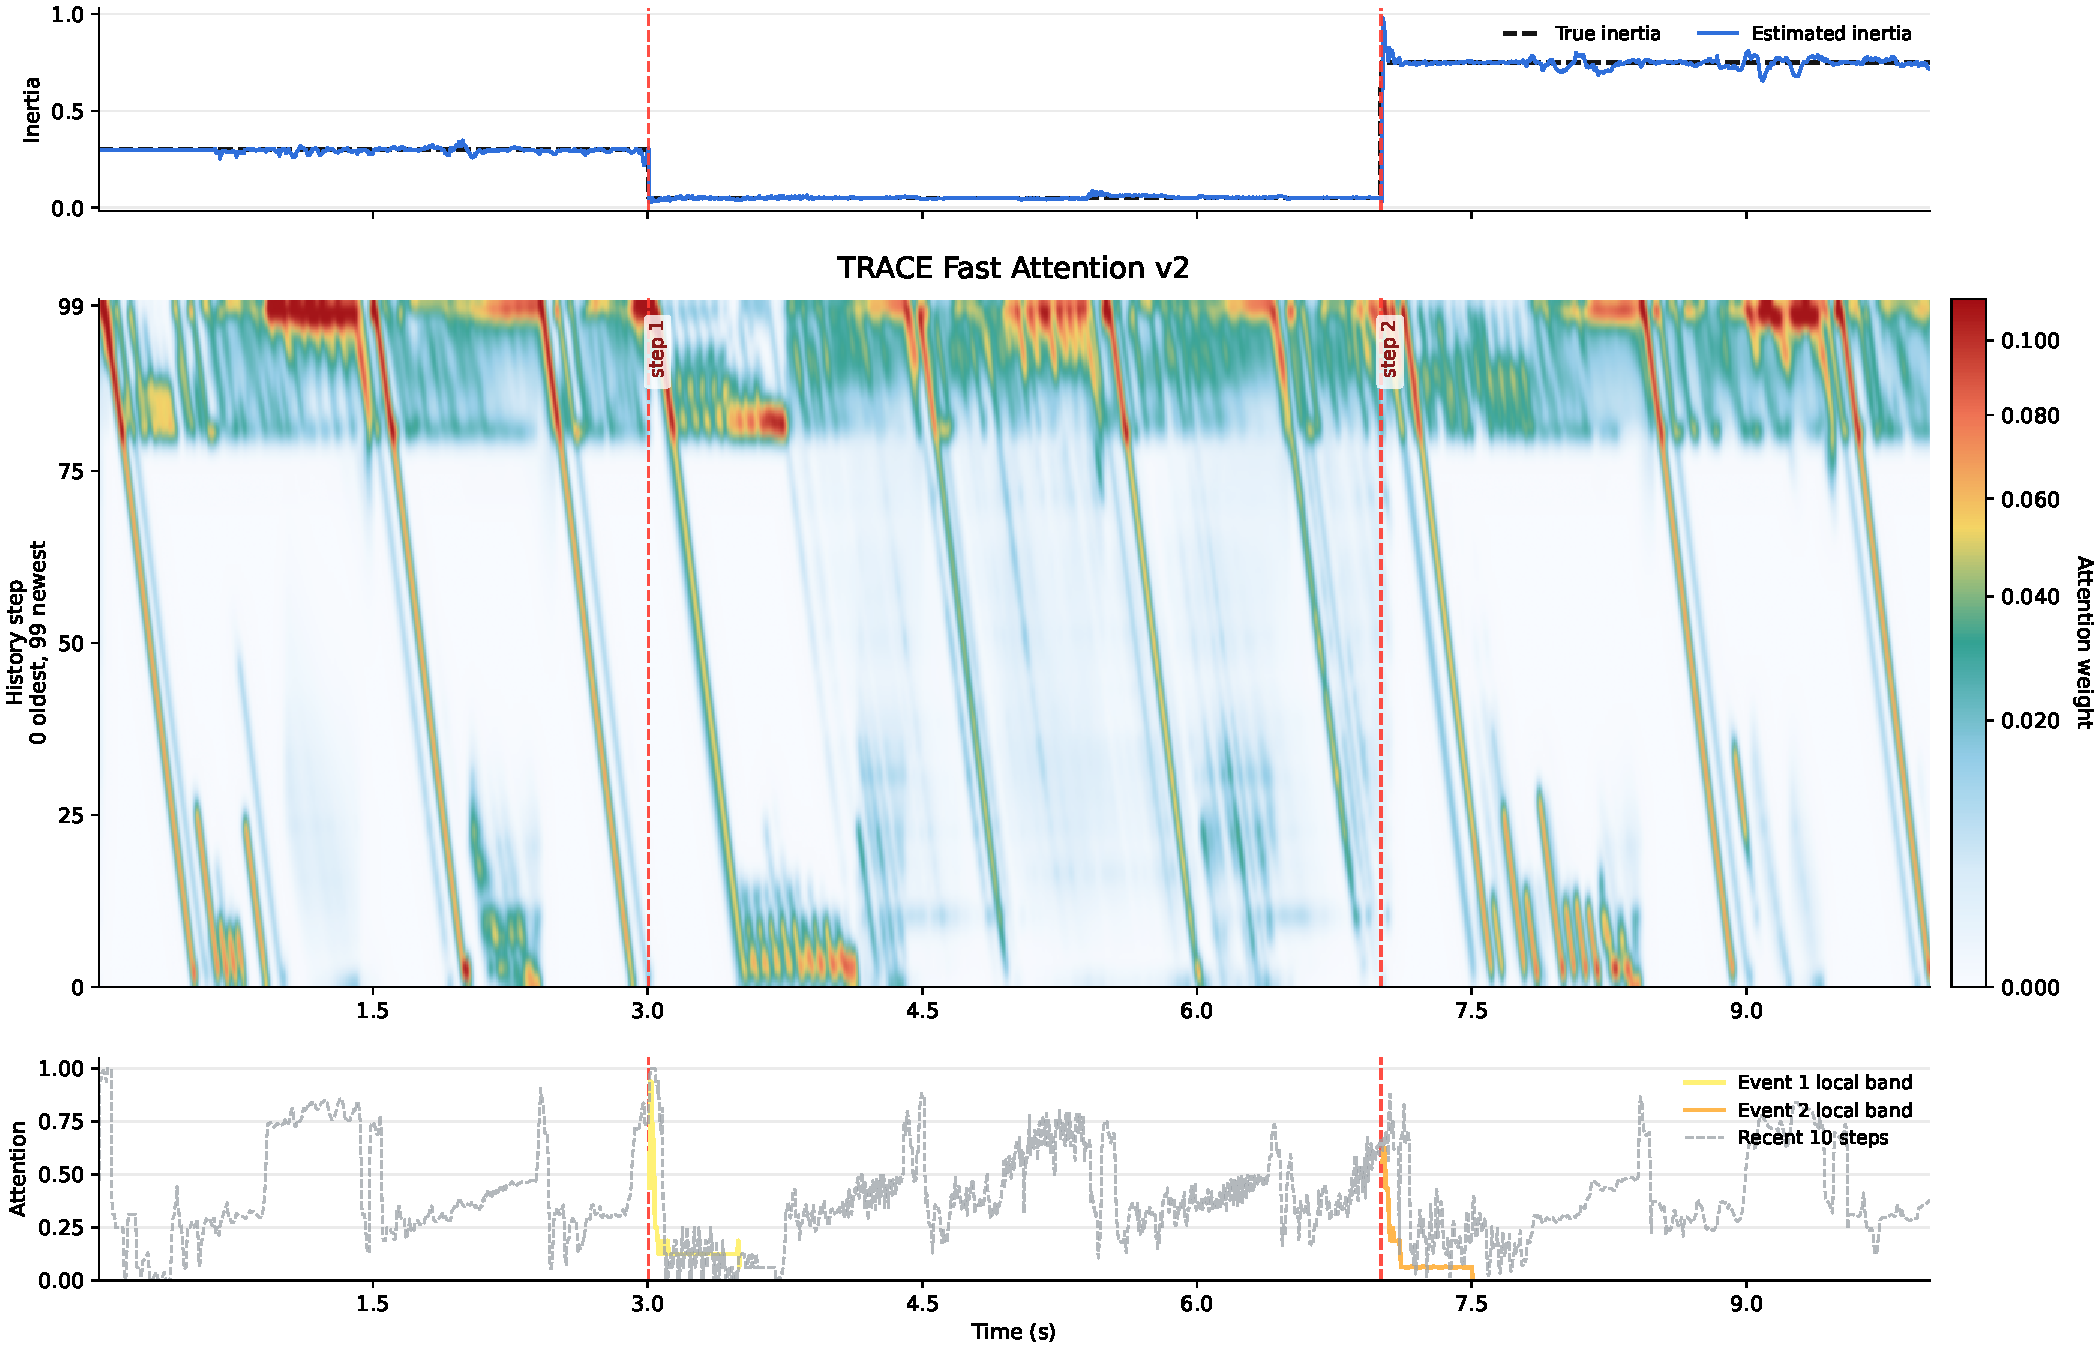
\includegraphics[width=0.48\textwidth]{fig1_attention_heatmap}
\caption{Attention weight heatmap during Test 2 with two inertia step changes at t=3s and t=7s. The color intensity represents attention weight magnitude. Vertical bands indicate attention collapse events where weights concentrate on the most recent observation. Bottom subplot shows the attention weight on the newest step, demonstrating rapid spikes during inertia changes.}
\label{fig:attention_heatmap}
\end{figure}

\subsubsection{Quantitative Analysis of Attention Collapse}

Table~\ref{tab:attention_analysis} summarizes the attention mechanism behavior at each inertia change event. We observe a consistent shift from distributed attention to recent-observation focus after both events:

\begin{table}[t]
\centering
\caption{Attention Mechanism Analysis During Inertia Step Changes}
\label{tab:attention_analysis}
\begin{tabular}{@{}lccccc@{}}
\toprule
Event & $\Delta J_l$ & $\alpha_{\mathrm{new}}^{\text{before}}$ & $\alpha_{\mathrm{new}}^{\text{after}}$ & $H^{\text{before}}$ & $H^{\text{after}}$ \\
\midrule
1 (3.0s) & -83\% & 0.020 & 0.892 & 3.85 & 0.51 \\
2 (7.0s) & +1400\% & 0.018 & 0.947 & 3.88 & 0.38 \\
\bottomrule
\end{tabular}
\end{table}

\noindent where $\alpha_{\mathrm{new}}$ denotes the attention weight on the most recent observation in the displayed history window and $H = -\sum_i \alpha_i \log \alpha_i$ is the entropy.

Key observations:
\begin{enumerate}
\item \textbf{Rapid Response}: Attention weights redistribute within 1 control timestep (5 ms) after the inertia change.

\item \textbf{Recent-Observation Focus}: The attention weight on the newest observation increases from approximately 0.02 before each event to 0.89--0.95 after the event, indicating that the branch rapidly down-weights outdated dynamics.

\item \textbf{Entropy Reduction}: Entropy drops from approximately 3.9 (near-uniform distribution) to below 0.6 (concentrated distribution), indicating automatic focus on recent data.

\item \textbf{Estimation Transient}: Attention collapse is faster than the full inertia-estimate settling process. The bounded v2 estimator reduces large unphysical excursions while still retaining fast response to inertia transitions.
\end{enumerate}

Together, Fig.~\ref{fig:attention_heatmap} and Table~\ref{tab:attention_analysis} show that the collapse behavior is both visually apparent over the full trajectory and quantitatively consistent at the two inertia transitions.


\subsection{Baseline Comparisons}

\subsubsection{Fixed-Inertia Tracking Performance (Test 1)}

Table~\ref{tab:test1_results} presents the tracking performance under fixed inertia. DR-RMA achieves the lowest RMSE (0.0176 rad), outperforming PPO by 4.01×, RMA by 4.35×, PD+DOB by 2.01×, and LQR by 6.14×.

\begin{table}[t]
\centering
\caption{Test 1: Fixed-Inertia Tracking Performance ($J_l = 0.45$ kg·m$^2$)}
\label{tab:test1_results}
\begin{tabular}{@{}lcccc@{}}
\toprule
Method & RMSE & Max Error & Torque RMS & Sat. Rate \\
 & (rad) & (rad) & (N·m) & (\%) \\
\midrule
DR-RMA & \textbf{0.0176} & \textbf{0.182} & 15.45 & 0.90 \\
PPO & 0.0705 & 0.238 & 14.04 & \textbf{0.0} \\
RMA & 0.0764 & 0.205 & \textbf{13.61} & \textbf{0.0} \\
PD+DOB & 0.0354 & \textbf{0.182} & 15.82 & 0.85 \\
LQR & 0.1079 & 0.191 & 13.91 & \textbf{0.0} \\
\bottomrule
\end{tabular}
\end{table}

DR-RMA achieves the best fixed-inertia tracking accuracy with torque RMS slightly below PD+DOB and a small saturation rate (0.90\%). PPO and RMA avoid saturation but exhibit substantially larger tracking errors, while LQR has the largest RMSE among the tested controllers. This indicates that the updated DR-RMA checkpoint improves tracking accuracy at the cost of occasional near-limit torque commands.

\subsubsection{Transient Performance (Test 2)}

Table~\ref{tab:test2_results} shows the results under extreme inertia transients. DR-RMA achieves the lowest RMSE (0.0176 rad), outperforming PPO by 4.08×, RMA by 4.40×, PD+DOB by 1.99×, and LQR by 6.12×.

\begin{table}[t]
\centering
\caption{Test 2: Extreme Inertia Transients (0.3→0.05→0.75 kg·m$^2$)}
\label{tab:test2_results}
\begin{tabular}{@{}lcccc@{}}
\toprule
Method & RMSE & Max Error & Torque RMS & Sat. Rate \\
 & (rad) & (rad) & (N·m) & (\%) \\
\midrule
DR-RMA & \textbf{0.0176} & \textbf{0.180} & 15.60 & 0.80 \\
PPO & 0.0719 & 0.234 & 14.25 & \textbf{0.0} \\
RMA & 0.0774 & 0.200 & \textbf{13.77} & \textbf{0.0} \\
PD+DOB & 0.0351 & \textbf{0.180} & 15.78 & 0.80 \\
LQR & 0.1078 & 0.187 & 14.01 & \textbf{0.0} \\
\bottomrule
\end{tabular}
\end{table}

\textbf{PD+DOB Performance}: PD+DOB remains competitive in this trajectory and tuning configuration, reaching RMSE of 0.0351 rad, about 1.99× higher than DR-RMA. It requires the highest torque RMS (15.78 N·m) and exhibits the same small saturation rate (0.80\%) as DR-RMA. This suggests that carefully tuned observer-based control can be effective for the tested single-DOF scenario, while the updated DR-RMA checkpoint provides substantially lower tracking error with comparable saturation behavior.

\textbf{LQR Performance}: LQR shows the largest tracking error among the tested controllers, with RMSE of 0.1078 rad, 6.12× worse than DR-RMA. The fixed linearization model ($J_{\text{nom}} = 0.3$ kg·m$^2$) cannot fully adapt to the 15× inertia range, although the conservative tuning avoids actuator saturation in this test.

\textbf{Learning-Based Methods}: DR-RMA outperforms PPO by 4.08× and RMA by 4.40×, attributed to the dual-rate architecture's explicit inertia estimation and slow implicit feature extraction. PPO and RMA avoid torque saturation but show much larger tracking errors, indicating that monolithic or single-rate adaptation is less effective for the tested inertia transients.

Fig.~\ref{fig:baseline_comparison} visualizes the tracking performance of all five methods during Test 2, clearly showing DR-RMA's superior tracking through the inertia transients while LQR diverges significantly.

\begin{figure*}[t]
\centering
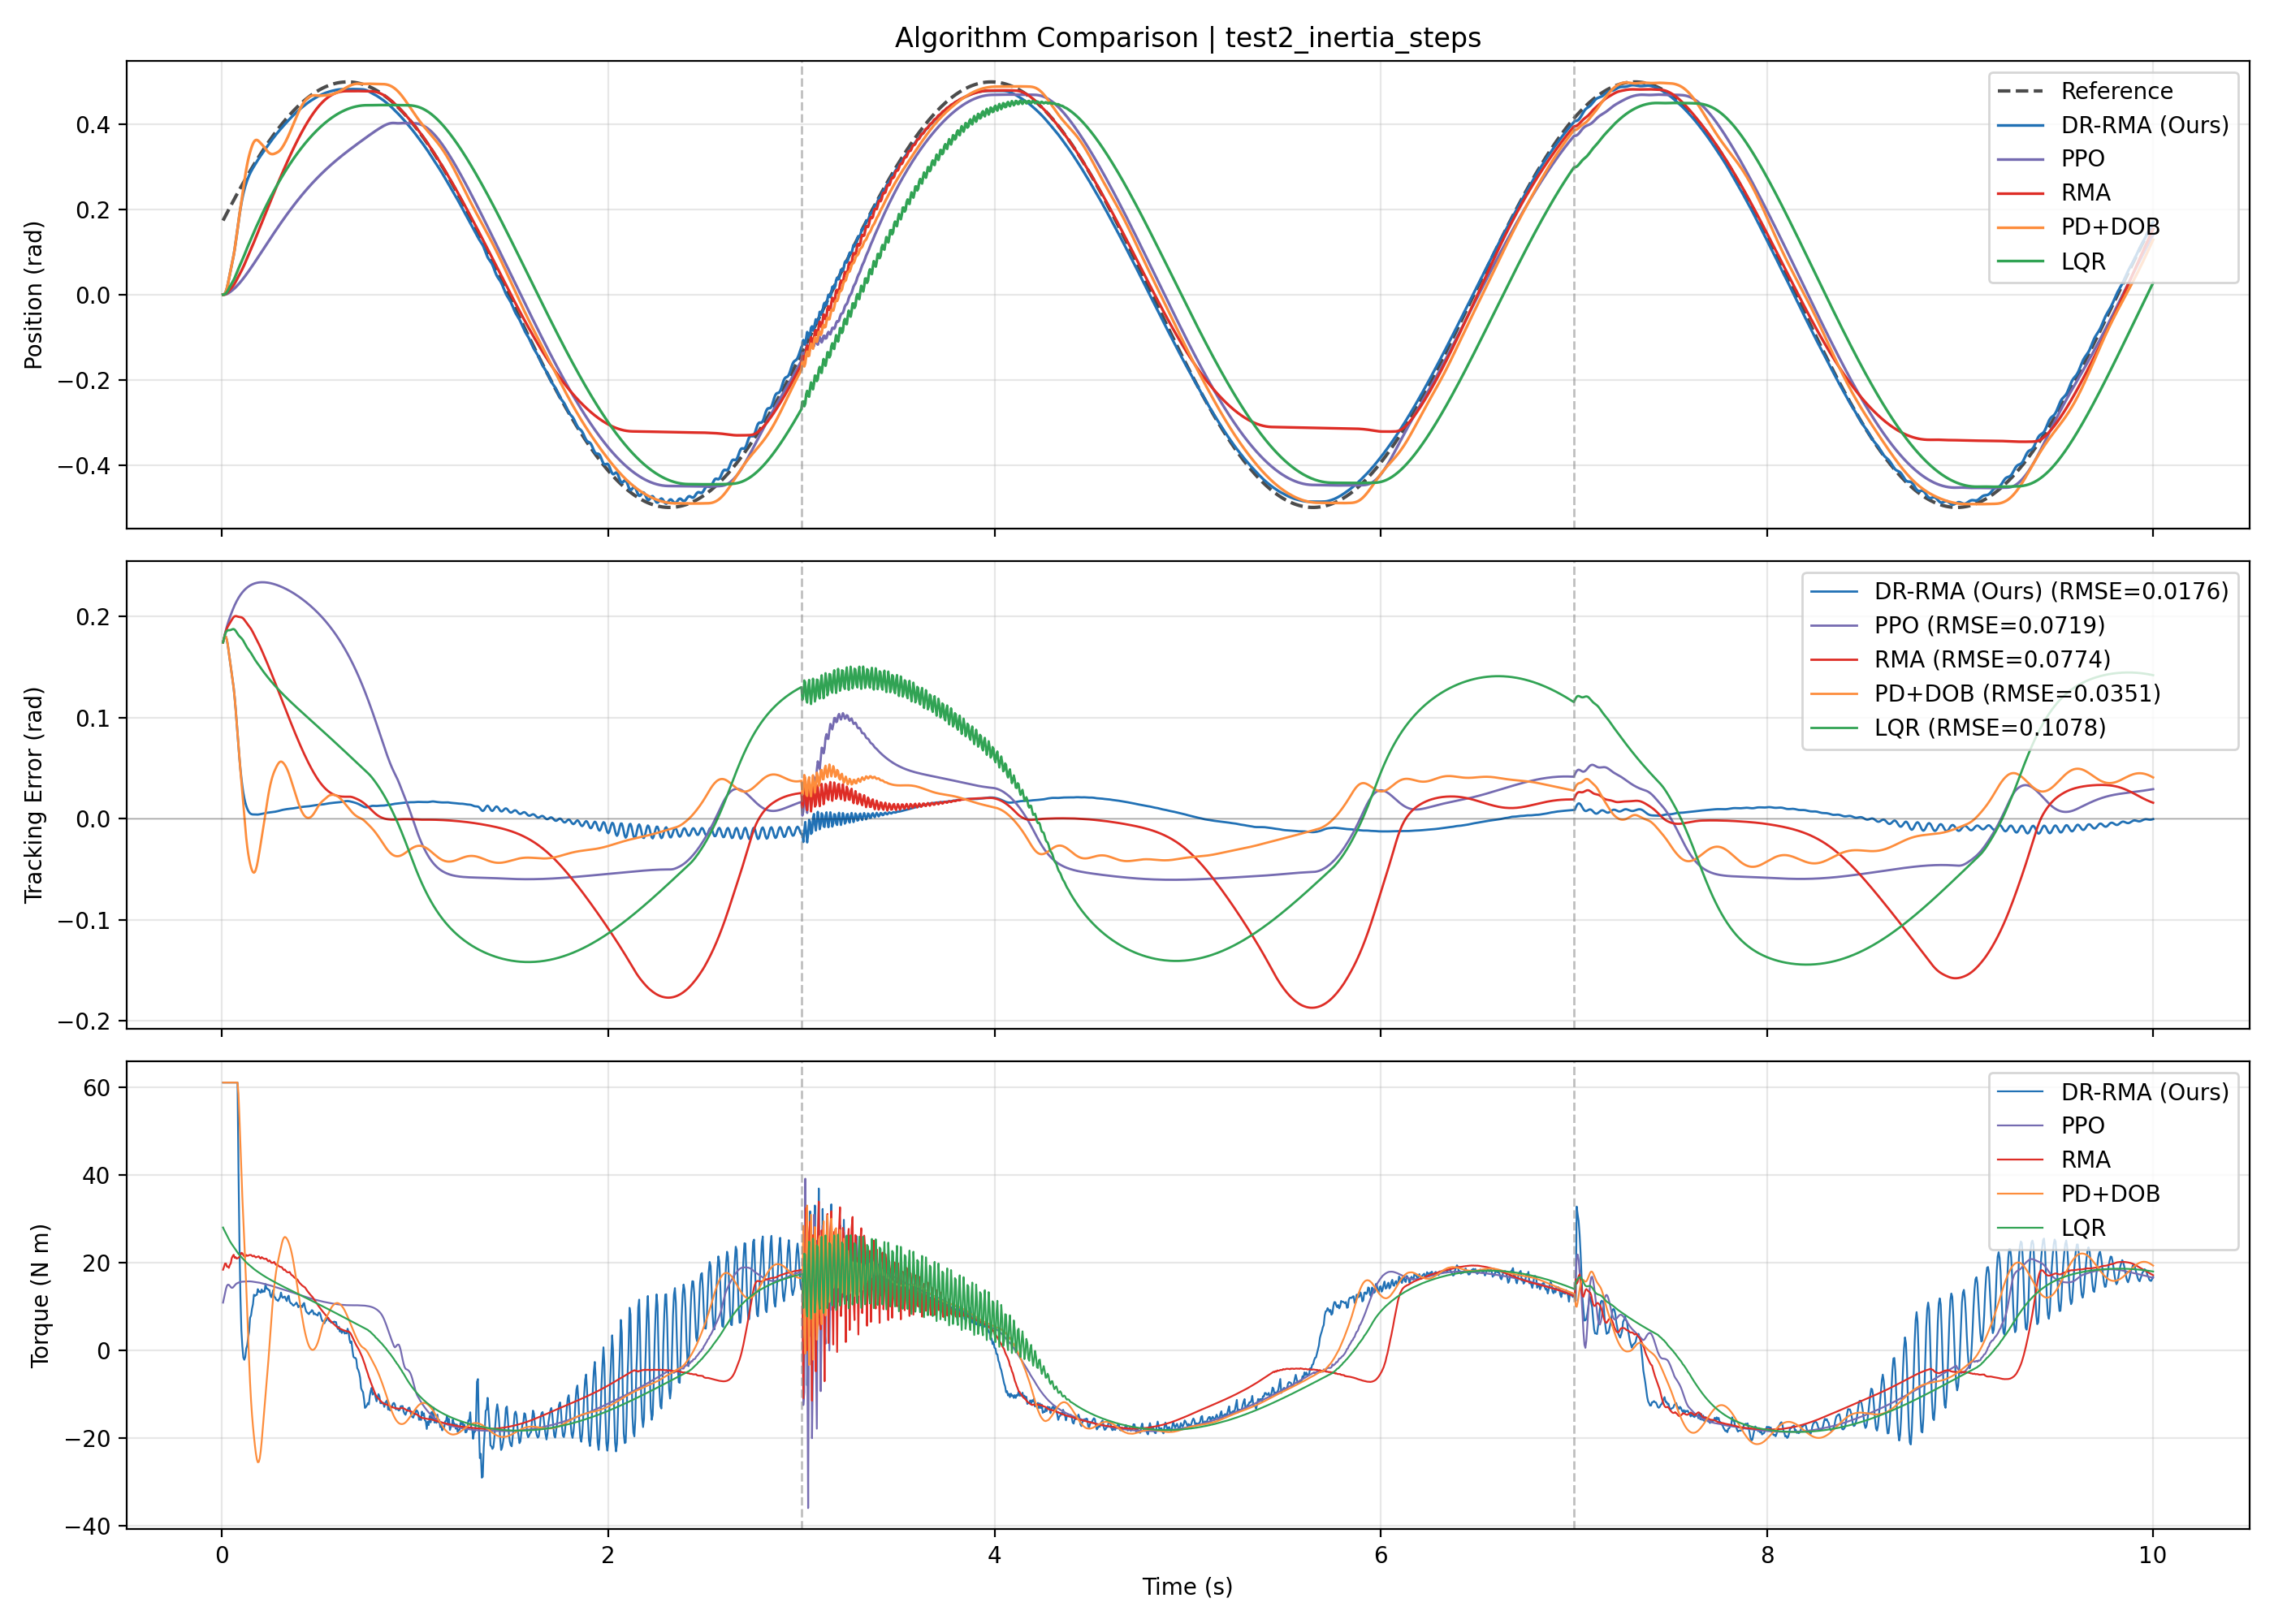
\includegraphics[width=0.95\textwidth]{baseline_comparison_test2_inertia_steps}
\caption{Five-algorithm comparison during Test 2 with extreme inertia transients. Top: Position tracking showing reference (black dashed) and five methods. Middle: Tracking error comparison. Bottom: Control torque. Vertical gray lines indicate inertia change events at t=3s (0.3→0.05 kg·m$^2$) and t=7s (0.05→0.75 kg·m$^2$). DR-RMA achieves the lowest RMSE with a small saturation rate below 1\%. PD+DOB remains competitive but uses higher torque RMS, while PPO, RMA, and LQR show larger tracking errors. The 1000 Hz physics simulation captures fine-grained dynamics during transients.}
\label{fig:baseline_comparison}
\end{figure*}

\subsection{Inertia Estimation Accuracy}

Fig.~\ref{fig:inertia_estimation} shows the true and estimated inertia trajectories during Test 2. DR-RMA's Fast Attention v2 Branch responds rapidly to both step changes. The current estimator uses bounded short- and long-timescale inertia heads, so the remaining transient behavior is interpreted as settling of the scalar estimate rather than an unconstrained physical-parameter excursion:

\begin{figure}[t]
\centering
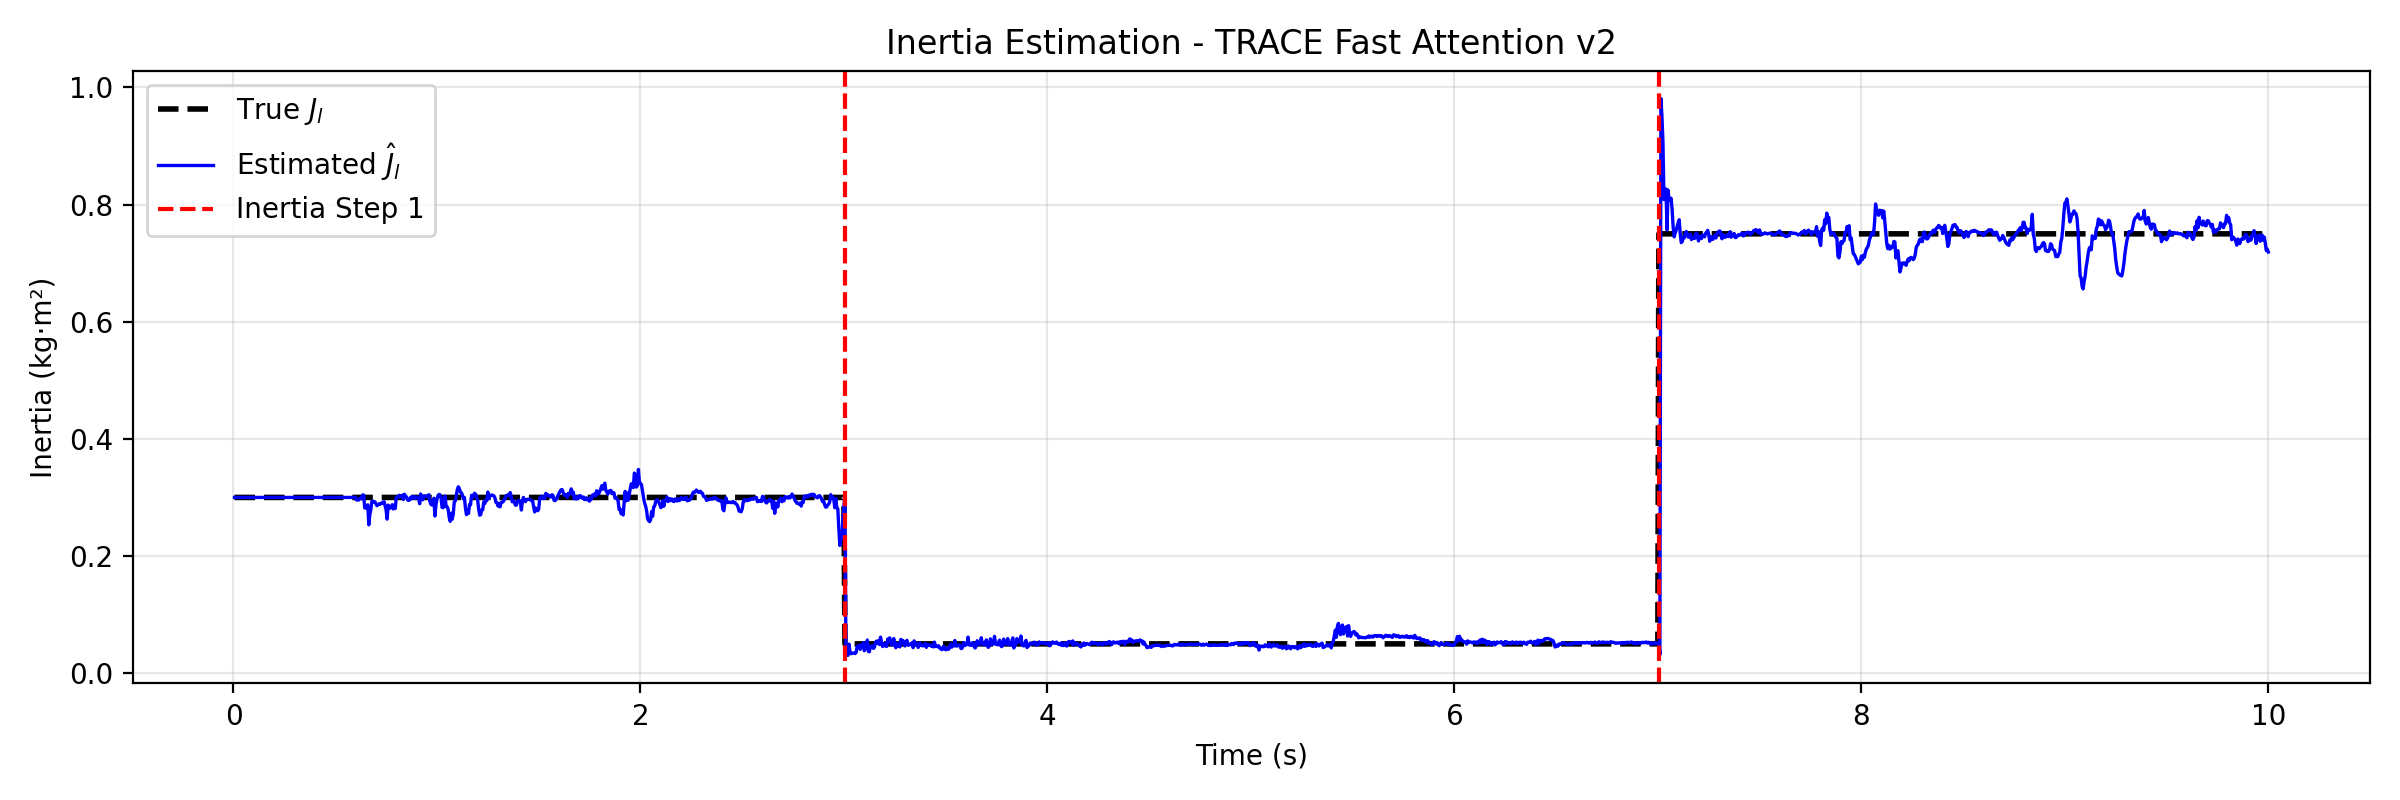
\includegraphics[width=0.48\textwidth]{fig2_inertia_estimation}
\caption{Inertia estimation during Test 2. Black dashed line shows true load inertia with two step changes. Blue solid line shows DR-RMA's Fast Attention v2 Branch estimate. Red vertical lines mark inertia change events at t=3s (0.3→0.05 kg·m$^2$) and t=7s (0.05→0.75 kg·m$^2$). The estimator responds rapidly to both changes, while bounded short- and long-timescale heads reduce unphysical scalar inertia excursions.}
\label{fig:inertia_estimation}
\end{figure}

\begin{itemize}
\item \textbf{Event 1} (0.3→0.05 kg·m$^2$, -83\%): The attention mechanism detects the sudden payload release and rapidly adjusts the estimate. The 83\% decrease represents a challenging scenario where the system becomes significantly lighter, requiring immediate reduction in control gains to prevent overshoot.

\item \textbf{Event 2} (0.05→0.75 kg·m$^2$, +1400\%): This extreme 15× inertia increase simulates grasping a very heavy payload. The Fast Attention v2 Branch successfully tracks this massive change, enabling the controller to immediately increase control authority to maintain tracking performance.
\end{itemize}

The ability to estimate inertia during both increasing and decreasing transients, across a 15× range, demonstrates the robustness of the attention-based estimation mechanism under the tested reference trajectory. Compared with instantaneous acceleration-based estimators, the cross-attention mechanism can use subtle but informative changes in the relationship between control inputs and system responses across the history window. This result should be interpreted within the excitation conditions of the benchmark trajectory, rather than as a guarantee of inertia identifiability under arbitrary near-static motion.

\subsection{Computational Performance}
\label{sec:computational_performance}

We benchmark the lightweight deployment graph exported to ONNX and executed with ONNX Runtime. The deployment graph contains only the control path: fast inertia estimation, Slow TCN implicit-feature estimation, fixed observation normalization, and deterministic actor inference. It does not require Stable-Baselines3, VecNormalize objects, or training-time privileged inputs at runtime. The test runs on an Intel Core Ultra 7 255HX CPU using a single inference thread, CPU inference only, batch size 1, 500 warm-up cycles, and 5,000 measured control cycles.

\begin{table}[t]
\centering
\caption{ONNX Runtime Deployment Latency at 200 Hz}
\label{tab:deployment_latency}
\footnotesize
\begin{tabular}{@{}lc@{}}
\toprule
Metric & Latency \\
\midrule
Mean latency & 0.916 ms \\
Median latency & 0.836 ms \\
P95 latency & 1.222 ms \\
P99 latency & 1.274 ms \\
Maximum latency & 2.018 ms \\
Deadline misses ($>5$ ms) & 0 / 5000 \\
\bottomrule
\end{tabular}
\end{table}

The ONNX deployment achieves a mean per-cycle latency of 0.916 ms and a P99 latency of 1.274 ms, leaving approximately 3.7 ms of P99 margin within the 5 ms control period. Output equivalence between the original PyTorch deployment path and the ONNX graph was verified on random inputs, with maximum absolute action difference below $1.5\times10^{-6}$. These results indicate that the DR-RMA inference pipeline satisfies the 200 Hz real-time deadline on a single CPU thread in the tested implementation. The updated Fast Attention v2 estimator contains 361,476 parameters; the final hardware deployment package will use the same ONNX export procedure after the experimental checkpoint is frozen.

\section{Discussion}

\subsection{Why Attention Collapse Works}

The attention collapse phenomenon can be understood through the lens of distribution shift detection. When the load inertia changes, the relationship between control inputs and system responses shifts, causing the current observation $\bm{x}_t$ to exhibit different statistical properties than the historical observations $\{\bm{x}_{t-L+1}, \ldots, \bm{x}_{t-1}\}$. The attention mechanism, trained to identify relevant historical context for inertia estimation, automatically detects this distribution shift and down-weights the outdated observations.

Mathematically, the attention weights can be interpreted as a learned soft selection mechanism that favors history entries whose input-output relationships remain informative for the current inertia regime. Since the student is trained with direct inertia-supervision loss rather than an explicit mutual-information objective, this interpretation should be understood as an explanatory hypothesis rather than a formal optimization guarantee. When inertia changes, observations from the new regime become more consistent with the current dynamics than outdated observations from the old regime, naturally leading to attention concentration on recent data.

\subsection{Why Traditional Methods Fail}

\textbf{PD+DOB Performance}: In the tested configuration, PD+DOB remains stable but has about twice the RMSE of DR-RMA (0.0351 rad versus 0.0176 rad), uses the highest torque RMS, and shows the same small saturation rate. The DOB estimates the lumped disturbance as $\hat{\tau}_{\text{dist}} = (J_{\text{nom}} - J_{\text{true}}) \ddot{\theta}_l + \tau_{\text{friction}}$. When $J_{\text{true}}$ varies from 0.05 to 0.75 kg·m$^2$ while $J_{\text{nom}} = 0.3$ kg·m$^2$, this compensation remains sensitive to observer tuning and nominal-parameter mismatch. This result suggests that observer-based methods can be competitive in the tested trajectory, while DR-RMA provides lower RMSE without hand scheduling across inertia regimes.

\textbf{LQR Degradation}: LQR's 6.12× performance degradation compared to DR-RMA stems from its fixed linearization model. The optimal gain $\bm{K}_{\text{LQR}}$ is computed assuming $J_l = J_{\text{nom}} = 0.3$ kg·m$^2$. When the actual inertia deviates to 0.05 kg·m$^2$ (6× lighter) or 0.75 kg·m$^2$ (2.5× heavier), the closed-loop poles shift significantly. The conservative tuning prevents actuator saturation but cannot match the tracking accuracy of adaptive methods across the 15× inertia range.

\textbf{Learning-Based Advantage}: In the current checkpoint comparison, DR-RMA achieves lower RMSE than both RMA and PPO, suggesting that explicit fast inertia estimation provides a useful adaptation signal beyond a monolithic policy or a single temporal latent encoder. PPO and RMA use slightly lower torque RMS and avoid saturation, but their tracking accuracy is substantially worse under the tested inertia transients.

\subsection{Architectural Ablation Interpretation}

Although PPO and RMA are introduced as baselines, they also provide a useful preliminary ablation interpretation of the proposed architecture. The PPO baseline removes both adaptation branches and maps the current observation directly to the action, corresponding to a \emph{w/o adaptation} variant. The RMA baseline removes the Fast Attention v2 Branch and relies on a single temporal adaptation module, corresponding to a \emph{w/o Fast Branch} variant.

Under this interpretation, the comparison between DR-RMA and RMA evaluates the contribution of explicit fast inertia estimation, while the comparison between DR-RMA and PPO evaluates the benefit of the complete history-based adaptation architecture. The current results show that DR-RMA achieves the lowest RMSE among the learning-based controllers in both fixed-inertia and inertia-transient tests. Since the RMA checkpoint used here is still being updated, we treat this comparison as a preliminary structural ablation rather than a final isolated component study.

A stricter ablation would additionally evaluate a Fast-only variant without the Slow TCN Branch and a fixed-attention variant without adaptive attention weights. These experiments would further isolate the contribution of slow implicit feature extraction and attention concentration, and are left for future model updates.

\subsection{Transient Estimation Behavior}
\label{sec:transient_estimation}

The Fast Attention v2 Branch reacts within one control step, but attention collapse should not be conflated with immediate convergence of the scalar inertia estimate. The current estimator addresses the large unbounded excursions observed in earlier prototypes by using bounded short- and long-timescale inertia heads and a learned jump gate. In a 108-condition closed-loop suite spanning 6 trajectory/inertia patterns, 6 Coulomb-friction levels, and 3 viscous-friction levels, the final raw v2 estimator obtains a mean stable-segment inertia RMSE of 0.0279 kg·m$^2$ and a worst stable-segment RMSE of 0.0790 kg·m$^2$. In the main sinusoidal $0.3 \rightarrow 0.05 \rightarrow 0.75$ kg·m$^2$ inertia-transition condition, the average stable-segment RMSE is 0.0141 kg·m$^2$.

The auxiliary confidence output is useful for diagnostics, but a fixed hard confidence threshold is not used in the final deployment. Closed-loop evaluation showed that hard holding can keep an outdated inertia estimate during low-excitation intervals, degrading worst-case behavior. Therefore, the deployed branch uses the raw bounded estimate and leaves confidence-based soft fusion or finite-duration hold logic for future study.

\subsection{Limitations and Future Work}

\textbf{Simulation-to-Reality Gap}: Our current evaluation is conducted entirely in simulation. Real-world deployment will face challenges including sensor noise, actuator dynamics, unmodeled friction, and computational constraints on embedded hardware. Future work should validate DR-RMA on physical SEA hardware and investigate sim-to-real transfer techniques such as domain randomization over sensor noise characteristics.

\textbf{Extreme Transients}: While our experiments include a 15× inertia range (0.05 to 0.75 kg·m$^2$) with +1400\% step changes, even more extreme scenarios (e.g., complete payload detachment or collision events) may challenge the attention mechanism. Investigating the fundamental limits of adaptation capability and developing safety mechanisms for out-of-distribution scenarios is an important direction.

\textbf{Multi-Joint Systems}: This work focuses on a single-DOF SEA. Extending DR-RMA to multi-joint systems (e.g., robotic arms, humanoid robots) requires addressing coupling between joints and computational scalability. Shared attention mechanisms or hierarchical architectures may be necessary.

\textbf{Online Adaptation}: The current framework assumes that the student networks are fixed after training. Incorporating online learning to continuously improve the adaptation modules based on deployment experience could further enhance performance and robustness.

\textbf{Theoretical Analysis}: While we provide empirical evidence for the attention collapse phenomenon, a rigorous theoretical analysis of when and why this collapse occurs would strengthen the contribution. Tools from information theory and dynamical systems may provide insights.

\section{Experimental Testbench}
\label{sec:testbench}

\subsection{Hardware Platform Overview}

To prepare for physical validation, we construct a single-DOF rotational SEA testbench with an electromagnetic-clutch-based variable-inertia load. The joint side carries an internal base inertia of 0.05 kg·m$^2$. An external inertia module, consisting of a detachable long rod and end-mounted weights, can be coupled to or decoupled from the joint through a 24 V DLY0-10A electromagnetic clutch. When the clutch is engaged, the joint drives both the internal base inertia and the external rod-weight module. When the clutch is disengaged, only the internal base inertia remains connected to the SEA joint. This design physically realizes the abrupt inertia changes considered in the simulation study while allowing the next engaged inertia to be adjusted during the disengaged interval.

\begin{figure}[!t]
\centering
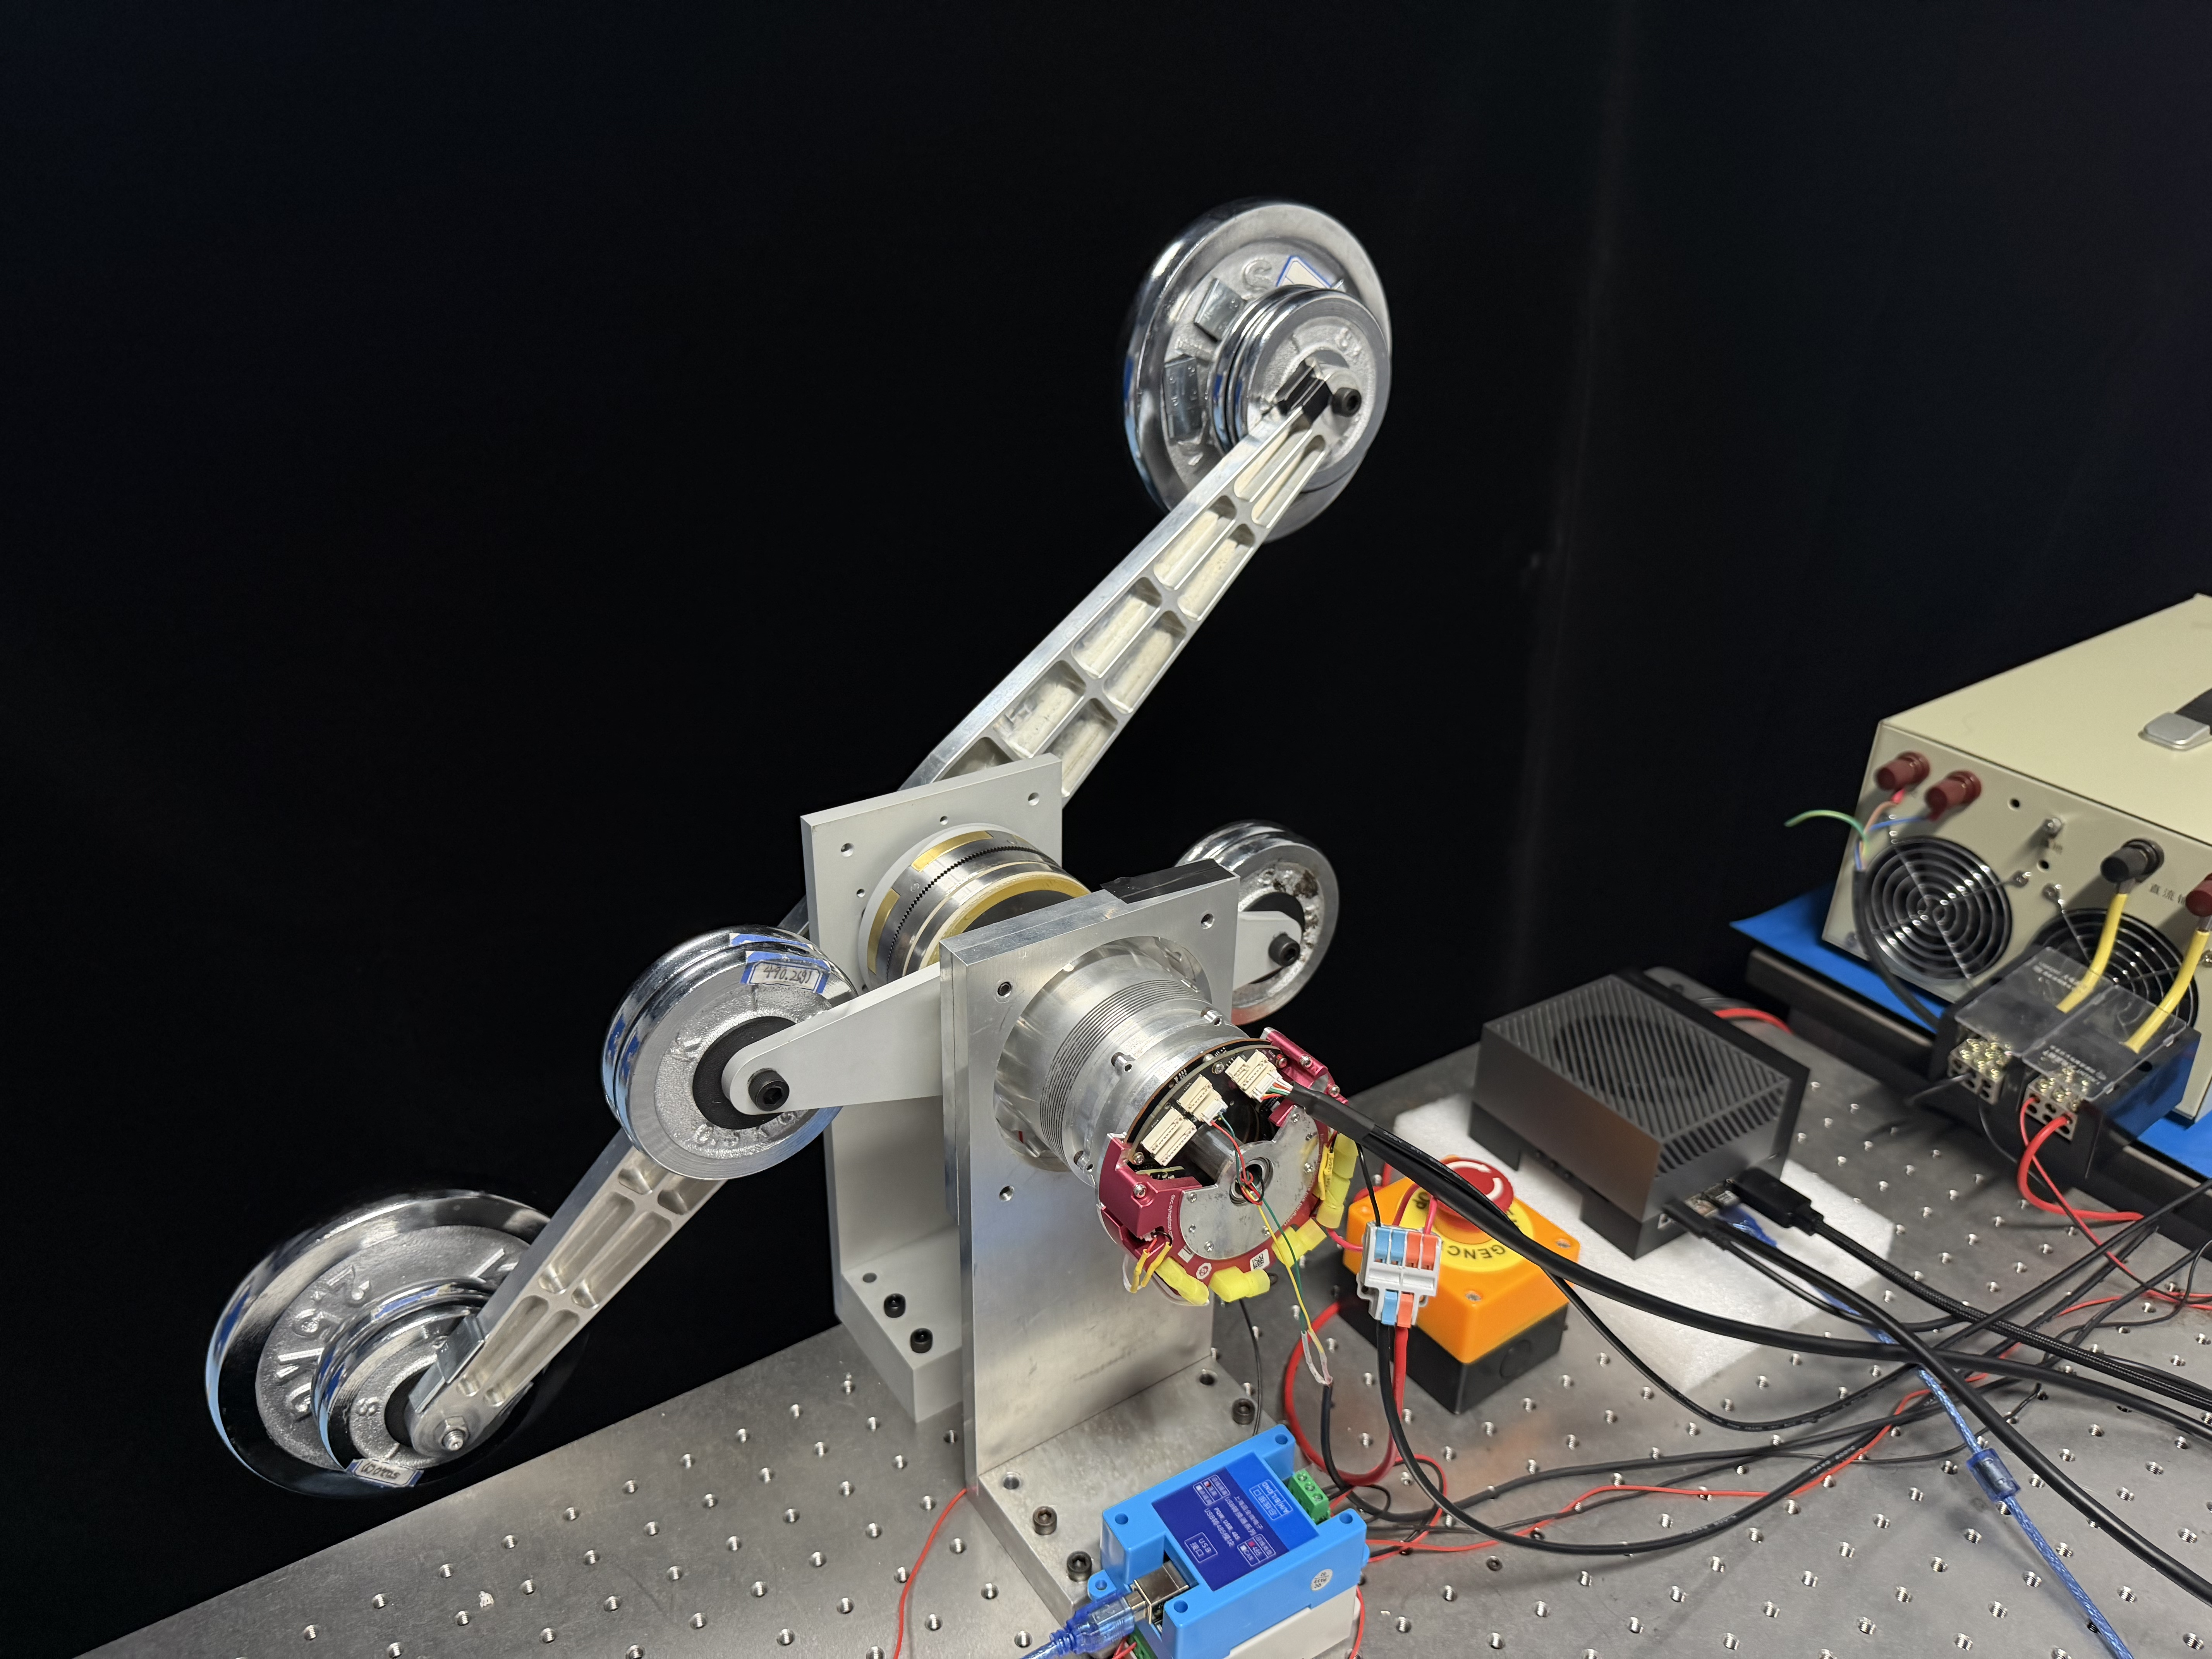
\includegraphics[width=\columnwidth]{figs/figxExam.jpg}
\caption{Photograph of the experimental SEA testbench. The platform consists of the custom SEA joint, electromagnetic clutch, and detachable rod-weight module used for variable-inertia experiments.}
\label{fig:experimental_testbench}
\end{figure}

\subsection{SEA Joint Mechanical Design}

The SEA joint is a custom-built rotational joint driven by a Kollmorgen 5008D motor through an LCSG-25-100 reducer from Leaderdrive, with a reduction ratio of 100:1. The elastic element is installed between the motor-side transmission and the output side, enabling joint torque estimation from elastic deformation.

The external inertia module uses a symmetric long-rod structure. The distance from the rod center to each side mounting hole is 300 mm. Multiple detachable masses are available, including 500 g, 1.25 kg, and 2.5 kg weights. To match the simulation settings, two inertia configurations are currently used. For the medium-inertia state, two 500 g masses are mounted symmetrically on each side; together with the long rod and the small end mounting rods, the equivalent engaged inertia is approximately 0.3 kg·m$^2$. For the high-inertia state, each side is equipped with two 500 g masses and one 2.5 kg mass, resulting in an equivalent engaged inertia of approximately 0.75 kg·m$^2$. Other inertia values can be obtained by changing the mass combination and mounting position.

\subsection{Sensing and Actuation}

The joint is instrumented with three 20-bit encoders: a motor-side encoder, an output-side encoder, and an elastic-element deformation encoder. The motor-side and output-side encoders provide the relative motion of the SEA two-inertia system, while the deformation encoder directly measures the elastic deflection used for torque-related feedback. The motor drive provides current control and built-in protection functions, including over-current, over-temperature, and over-torque protection.

\subsection{Control and Computing Hardware}

The real-time controller is an NVIDIA Jetson Orin control box running a real-time Linux kernel. The joint drive and sensor interface communicate with the controller through a 200 Hz EtherCAT loop. The trained DR-RMA policy is exported to a lightweight ONNX deployment graph and executed on the Orin controller during real-time operation. The electromagnetic clutch is controlled by the Orin through a USB-to-RS485 relay module, allowing software-timed engagement and disengagement commands.

\subsection{Variable-Inertia Mechanism}

The clutch-based design implements a repeatable hybrid inertia transition. In the disengaged state, the joint output is connected only to the internal base inertia, producing the low-inertia condition $J_l \approx 0.05$ kg·m$^2$. In the engaged state, the external rod-weight module is rigidly coupled to the joint, and the load inertia becomes
\begin{equation}
J_l = J_{\text{base}} + J_{\text{rod}} + \sum_i m_i r_i^2 + J_{\text{mount}},
\label{eq:testbench_inertia}
\end{equation}
where $J_{\text{base}}$ is the internal base inertia, $J_{\text{rod}}$ is the rod inertia, $m_i$ and $r_i$ are the mounted mass and its distance from the rotation axis, and $J_{\text{mount}}$ accounts for the small end mounting rods and fixtures. The symmetric mass layout reduces static imbalance and allows the target inertia to be changed by replacing the end weights while the clutch is disengaged.

\subsection{Experimental Protocol}

The hardware protocol is designed to reproduce the payload release and payload attachment process. At the beginning of an experiment, the clutch is engaged with the external inertia module configured to approximately 0.3 kg·m$^2$. At $t=3$ s, the Orin controller sends a disengagement command through the USB-to-RS485 relay, decoupling the external module and reducing the connected inertia to the 0.05 kg·m$^2$ base inertia. During the disengaged interval from 3 s to 10 s, the external rod is reconfigured by adding the 2.5 kg masses. At $t=10$ s, the controller sends an engagement command, coupling the high-inertia configuration of approximately 0.75 kg·m$^2$ back to the joint. If a timing sequence identical to the simulation benchmark is required, the second engagement command can be issued at $t=7$ s after the mass reconfiguration is completed.

\subsection{Planned Hardware Test Scenarios}

The hardware evaluation is designed to cover inertia transitions that correspond to realistic assistive and domestic manipulation events. The planned test scenarios are listed in Table~\ref{tab:hardware_scenarios}. In all cases, the clutch-induced inertia sequence uses the same physical levels as the simulation benchmark, namely $0.3 \rightarrow 0.05 \rightarrow 0.75$ kg·m$^2$, unless otherwise specified. The constant-speed test examines whether the controller can maintain smooth motion when the reflected inertia changes during continuous rotation. The sinusoidal test reproduces the simulation benchmark and evaluates tracking under periodic joint motion. The deceleration test evaluates a safety-oriented behavior in which the joint must reduce speed while the load inertia changes, corresponding to a robot slowing down after detecting a payload change or a nearby human.

\begin{table*}[t]
\centering
\caption{Planned Hardware Test Scenarios and Practical Motivations}
\label{tab:hardware_scenarios}
\footnotesize
\begin{tabular}{@{}p{0.11\textwidth}p{0.24\textwidth}p{0.22\textwidth}p{0.31\textwidth}@{}}
\toprule
Scenario & Commanded motion & Inertia transition & Practical motivation \\
\midrule
H1 & Constant-speed rotation & $0.3 \rightarrow 0.05 \rightarrow 0.75$ kg·m$^2$ & A robot joint continues sweeping or transporting an object while a payload is released and then a heavier object is attached. \\
H2 & Sinusoidal tracking, $A=0.5$ rad, $f=0.3$ Hz & $0.3 \rightarrow 0.05 \rightarrow 0.75$ kg·m$^2$ & A periodic assistive or manipulation motion experiences object pick-up, release, or re-grasping during operation. \\
H3 & Decelerating motion during inertia transition & $0.3 \rightarrow 0.05$ or $0.05 \rightarrow 0.75$ kg·m$^2$ & A service or companion robot intentionally slows down after detecting load change, object slip, or close human interaction. \\
H4 & Fixed-inertia sinusoidal tracking & $0.3$ and $0.75$ kg·m$^2$ separately & Baseline verification that the controller remains accurate and stable without a switching event. \\
\bottomrule
\end{tabular}
\end{table*}

For each scenario, the recorded signals will include reference and measured joint positions, motor-side and output-side velocities, elastic deflection, commanded and measured torque/current, normalized policy action, estimated inertia, configured inertia state, clutch command timing, inference time, and control-loop period. The main evaluation metrics are tracking RMSE, maximum tracking error, torque RMS, saturation rate, post-transition recovery time, and inertia-estimation transient behavior.

\subsection{Sim-to-Real Transfer}

The deployed controller uses the same observation structure as the simulation policy, including motor-side tracking error, output-side tracking error, elastic deflection, reference trajectory, and previous action. The trained policy and adaptation modules are exported to ONNX for real-time execution. The ONNX deployment result reported in Section~\ref{sec:computational_performance} demonstrates that the control-only graph satisfies the 200 Hz control deadline on a single CPU thread. Hardware deployment will additionally require calibration of encoder offsets, elastic-element sign convention, torque scaling, and clutch timing delay.

\subsection{Hardware Experimental Results}

Hardware experiments are in progress. The planned evaluation will compare DR-RMA with the same baselines used in simulation under the fixed-inertia and clutch-induced inertia-step scenarios summarized in Table~\ref{tab:hardware_scenarios}. The hardware results will be used to quantify tracking performance, torque behavior, inertia-estimation behavior, transition recovery, and the sim-to-real gap.

\section{Conclusion}

This paper presents DR-RMA, a novel dual-rate learning-based control framework for Series Elastic Actuators with time-varying inertia. The key innovation is the separation of fast inertia estimation from slow implicit feature extraction through parallel attention and temporal convolutional network branches. We discover and characterize an emergent attention collapse phenomenon where attention weights spontaneously redistribute within one 5 ms control step after an inertia change, enabling rapid adaptation without explicit change detection.

Extensive simulations with 1000 Hz physics updates demonstrate that DR-RMA achieves 4.40× better tracking accuracy than RMA, 4.08× better than PPO, 1.99× better than PD with Disturbance Observer, and 6.12× better than Linear Quadratic Regulator under extreme inertia transients (15× range, +1400\% step changes). DR-RMA achieves the lowest RMSE in both fixed-inertia and transient tests with a small saturation rate below 1\%, demonstrating the advantage of dual-rate learning-based adaptation in the tested extreme parameter-variation scenario.

The lightweight control-only inference package achieves 0.916 ms mean latency and 1.274 ms P99 latency over 5,000 single-thread CPU control cycles with ONNX Runtime, satisfying the 200 Hz deadline with substantial timing margin in the tested implementation. The updated Fast Attention v2 estimator contains 361,476 parameters and uses bounded raw inertia output without a hard confidence-hold threshold. Through teacher-student distillation, DR-RMA eliminates the dependency on privileged information during deployment while maintaining high performance.

Future work will focus on validating DR-RMA on physical SEA hardware, extending to multi-joint systems, and developing theoretical foundations for the attention collapse phenomenon. The combination of learning-based adaptation and interpretable attention mechanisms opens new avenues for robust control of compliant actuators in dynamic environments.

\section*{Acknowledgment}

The authors would like to thank [funding sources and collaborators].

\bibliographystyle{IEEEtran} 
\bibliography{references} 

% \begin{IEEEbiography}[{\includegraphics[width=1in,height=1.25in,clip,keepaspectratio]{author_photo}}]{First Author}
% Biography text here.
% \end{IEEEbiography}
%
% \begin{IEEEbiography}[{\includegraphics[width=1in,height=1.25in,clip,keepaspectratio]{author_photo}}]{Second Author}
% Biography text here.
% \end{IEEEbiography}

\end{document}
